% interactcadsample_cn.tex
% Chinese version based on interactcadsample.tex

\documentclass[]{interact}

\usepackage[UTF8,scheme=plain,fontset=none]{ctex}
\setCJKmainfont{Noto Serif CJK SC}
\setCJKsansfont{Noto Sans CJK SC}
\usepackage{xcolor}
\usepackage[normalem]{ulem}
\DeclareRobustCommand{\reviewadd}[2]{{\color{red}#1}\ {\color{blue}\footnotesize[#2]}}
\DeclareRobustCommand{\reviewdel}[1]{{\color{gray}\sout{#1}}}
\usepackage{epstopdf}% To incorporate .eps illustrations using PDFLaTeX, etc.
\usepackage{subfigure}% Support for small, `sub' figures and tables
%\usepackage[nolists,tablesfirst]{endfloat}% To `separate' figures and tables from text if required
\usepackage{enumitem}
\usepackage{natbib}% Citation support using natbib.sty
\usepackage{amsmath}
\usepackage{multirow} 
\usepackage{algorithm}      
\usepackage{algorithmicx}   
\usepackage{algpseudocode}  
\usepackage{setspace}
\onehalfspacing  
\renewcommand{\abstractname}{摘\quad 要}
\renewcommand{\figurename}{图}
\renewcommand{\tablename}{表}
\renewcommand{\appendixname}{附录}
\renewcommand{\refname}{参考文献}
\renewcommand{\contentsname}{目\quad 录}
\renewcommand{\today}{\number\year 年\number\month 月\number\day 日}
\renewcommand\keywordsname{关键词}
\makeatletter
\gdef\@received{编译日期：\today}
\def\@maketitle{\thispagestyle{plain}
  \clearpage
  \null
  \bgroup
    \parindent0pt
    \vspace*{36pt}
    {\articletypefont{\@articletype}\par}%
    \vskip13pt
    {\titlefont{\@title}\par}%
    \vskip13pt
    {\authorfont\@author\par}%
    \ifsuppldata\else
    \vskip17pt
    {\receivedfont{\bfseries 文章历史\\}\@received\par}%
    \fi
    \vskip13pt
  \egroup}
\makeatother
\bibpunct[, ]{(}{)}{;}{a}{}{,}% Citation support using natbib.sty
\renewcommand\bibfont{\fontsize{10}{12}\selectfont}% Bibliography support using natbib.sty

\theoremstyle{plain}% Theorem-like structures provided by amsthm.sty
\newtheorem{theorem}{定理}[section]
\newtheorem{lemma}[theorem]{引理}
\newtheorem{corollary}[theorem]{推论}
\newtheorem{proposition}[theorem]{命题}

\theoremstyle{definition}
\newtheorem{definition}[theorem]{定义}
\newtheorem{example}[theorem]{例}

\theoremstyle{remark}
\newtheorem{remark}{注}
\newtheorem{notation}{记号}
%\providecommand{\replace}[2]{#2} 
\begin{document}

\articletype{论文模板}

\title{面向稳健参数设计中非平稳高斯过程建模的两阶段注意力引导主动学习}

\author{
	\name{冯泽彪\textsuperscript{a}\thanks{*通讯作者。邮箱：zbfeng@njupt.edu.cn}，杨旭\textsuperscript{a}，王建军\textsuperscript{b}，黄卫东\textsuperscript{a}}
	\affil{\textsuperscript{a}南京邮电大学管理学院，南京 210003，中国；\textsuperscript{b}南京理工大学管理科学与工程系，南京 210094，中国}
}

\maketitle

\begin{abstract}
稳健参数设计是工业实践中持续质量改进的重要方法。然而，在样本有限的条件下对非平稳响应面进行建模仍然具有挑战性，因为预测精度不足可能导致最优参数设置估计出现乐观偏差。本文在非平稳高斯过程（NSGP）建模框架下，提出一种面向稳健参数设计的两阶段注意力引导主动学习方法。该方法将 softmax 加权质量损失函数与 maximin 距离准则相结合，在潜在最优子区域的局部精度与全局空间填充之间取得平衡。第一阶段依据候选设计点与潜在最优子区域的相关性进行排序，并选取高权重子集进入后续筛选；第二阶段在该子集中进一步引入空间多样性约束，以缓解样本聚集。随后，将选取的样本点加入训练集并更新 NSGP 模型。本文进一步采用遗传算法求解基于 NSGP 的稳健参数设计问题，从而确定最优参数设置。\reviewadd{与多种经典实验设计方法和现代主动学习采集函数（含 Expected Improvement、Integrated Mean Squared Error reduction 和 Upper Confidence Bound）的广泛对比表明，}{R1-2, R2-4}所提方法能够在数据稀缺场景下提高预测精度，并增强优化解的稳健性。\reviewadd{通过消融实验、目标值敏感性分析和 10 维工程基准案例进一步验证了方法的有效性。}{R1-1, R2-1, R2-2, R2-6}
\end{abstract}

\begin{keywords}
质量工程；稳健参数设计；非平稳高斯过程建模；主动学习；两阶段注意力引导采集
\end{keywords}


\section{引言}
\subsection{研究动机}
在现代制造系统中，产品质量直接关系到企业竞争力、客户忠诚度和运营成本控制，也与市场份额和顾客满意度提升密切相关 \citep{Wu2011, He2021, Liw2025}。系统化质量改进还能够降低缺陷、返工和保修成本 \citep{Wu2020}。作为质量工程的重要方法，稳健参数设计（RPD）通过确定设计参数与工艺参数组合，降低系统对噪声因素的敏感性，从而提高质量特性的稳定性和一致性 \citep{Bao2016, Ouyang2016, Ouyang2025}。RPD 已广泛应用于先进制造、工程系统和服务运营，为不确定条件下的性能优化提供了理论支撑 \citep{Chuang2017, An2020, Huang2022}。响应面方法（RSM）通过统计方式近似输入—输出关系，是实施 RPD 的重要工具 \citep{Fan2000, Ding2004, Peterson2009, Li2025}。然而，现代工程系统的质量特性日益呈现高维、强非线性和显著非平稳等特征。在这类条件下，传统响应面模型或代理模型难以在有限数据下获得足够的精度和泛化能力，从而影响最优解的有效性和质量改进效率。

基于 Gaussian process（GP/Kriging）的代理建模因具有系统的不确定性量化能力和灵活的非线性函数逼近能力，已成为稳健优化中的核心技术之一 \citep{Williams2006, Ankenman2010, Santner2018, Liu2025}。主动学习提供了一种面向信息增益的实验设计范式，使有限数据条件下的数据高效 GP 建模和稳健优化成为可能 \citep{Wang2025, Feng2025}。不过，现有研究相当一部分仍建立在平稳性假设之上，并忽视对潜在最优区域附近子空间的定向探索，进而降低响应面建模效率并削弱优化解的稳健性。为弥补这一不足，本文在有限数据条件下提出一种面向 NSGP 建模和稳健参数设计的两阶段注意力引导主动学习框架。第一阶段采用 softmax 加权质量损失准则，优先提高潜在最优区域的预测精度；第二阶段采用 maximin 空间填充规则，抑制局部聚集并改善空间覆盖。最终，将注意力增强的 NSGP 嵌入稳健参数设计方案。

\subsection{相关研究工作}
近年来，已有大量文献研究基于 GP 建模的 RPD 方法 \citep{Jiang2021}。在应用与建模集成方面，\citet{Dellino2012} 将 Kriging、非线性规划和重采样策略结合，以缓解代理模型不确定性；\citet{Tan2012} 引入基于 Lugannani--Rice 鞍点近似的期望二次损失准则，提高优化可靠性。若干研究在 Bayesian 框架下推进多响应 GP 建模 \citep{Alshraideh2014, Kleijnen2014}；\citet{Li2016} 提出成对建模策略，\citet{Ding2024} 则发展了考虑协变量的 Gaussian process profile 模型，均旨在提高预测精度。\citet{Han2016}、\citet{Wang2019} 和 \citet{Wang2022} 分别通过闭式质量损失、IMSE 采样和输入位置误差分析处理输入不确定性。\citet{Feng2021} 提出用于异常值稳健优化的 Student-\emph{t} GP。\citet{Chen2022}、\citet{Barde2024} 和 \citet{Zhou2025} 分别利用 projection-pursuit additive Gaussian processes、稀疏变分 coregionalization 模型和 Dirichlet Gaussian processes 处理高维问题。尽管已有研究取得了进展，多数方法仍假设训练数据集固定，限制了设计点的自适应能力，也削弱了小样本条件下响应面模型的有效性。

在数据稀缺场景下，主动学习通过优先选择信息量高的样本提升数据效率和稳健性。\citet{Chen2021} 将 D-optimality 与 maximin 空间填充准则结合，以提高 GP 模型精度。\citet{Han2021} 基于轮廓估计提出控制变量与噪声变量协同采样的双采集策略。\citet{Zhang2024} 在 AK-Gibbs 方法中采用 Gibbs 重要性采样，以更好估计高维问题中的小失效概率。\reviewadd{在 Bayesian optimization 领域，Expected Improvement（EI）\citep{Jones1998}、Integrated Mean Squared Error reduction（IMSE）\citep{Sacks1989} 和 Upper Confidence Bound（UCB）\citep{Srinivas2010} 等采集函数已被广泛用于平衡 exploration 与 exploitation，}{R1-2, R2-4, R2-7}然而，这些方法通常依赖平稳性假设，限制了其刻画工业过程常见非平稳特征的能力。针对这一问题，已有多种 NSGP 模型被提出。\citet{Gramacy2008} 提出基于树分区的 NSGP，并有效刻画火箭助推器设计中的非平稳响应；\citet{Konomi2014} 将 NSGP 扩展到多输出系统，用于复杂流体动力学建模；\citet{Rhode2020} 在 NSGP 框架下评估多种置信带构造方法。Liu (2021) 通过结合 global--local GP 集成与滑动窗口排序机制提高预测精度。在统一建模与优化方面，\citet{Davis2021} 提出 Bayesian composite GP 模型，通过非恒定方差结构解耦全局趋势和局部波动；\citet{Meng2022} 构建组合框架，在多峰响应面中平衡全局探索与局部开发。Deep Gaussian processes（DGPs）也被用于非平稳函数建模。\citet{Sauer2022} 将 DGPs 引入主动学习，以近似数据稀缺场景下的复杂仿真；\citet{Gnanasambandam2024} 将 DGPs 与随机插补结合，提高多类基准函数和金属增材制造应用中的效率。不过，多数现有研究在主动学习过程中忽略潜在最优区域的预测精度，可能导致对所得解稳健性的过度估计。

注意力机制起源于深度学习中的自然语言处理，并已广泛应用于计算机视觉、时间序列预测、多任务优化以及科学计算代理建模 \citep{Yu2022}。其核心思想是对特征进行自适应加权，以突出与任务性能最相关的信息。在主动学习中，这一思想可以引导采样关注对响应或稳健性指标具有更大影响的区域，从而在有限数据下提高建模效率和预测精度。在 GP 建模中，注意力思想也被嵌入表示学习和推断过程。\cite{Li2022} 建立了 GP mixture 与注意力机制之间的联系，并提出适用于非欧式空间的变体；\cite{Xie2022} 提出基于 GP 的 channel attention 模块，以概率方式进行通道相关性建模；\cite{Zhong2024} 将 transformer 学习与 Gaussian attention 结合，用于提高木材表面缺陷分割效果，尤其适用于边界模糊和形态不规则的情形。尽管这些方法提高了模型精度，但通常采用单目标注意力机制，容易造成设计点局部聚集并降低采样策略的整体适应性。

为解决上述问题，本文提出一种面向有限数据稳健优化的两阶段注意力引导主动学习 NSGP 建模框架。第一阶段采用 softmax 加权质量损失采集准则，将采样聚焦于潜在最优子区域，从而提高局部预测精度；第二阶段采用 maximin 空间填充准则，抑制局部聚集并增强全局覆盖。由此得到的注意力增强 NSGP 代理模型进一步嵌入稳健参数设计模型。本文主要贡献如下：
\begin{enumerate}
	\item 构建了一个面向小样本与非平稳响应的注意力引导主动学习 NSGP 优化框架，同时提高非平稳性刻画能力和优化质量。
	\item 提出一种有原则的两阶段采集策略，将目标感知的质量损失评分与空间填充的 maximin 规则耦合，在潜在最优区域实现高效且保持多样性的采样。
	\item 设计了基于质量损失的目标驱动主动学习流程，增强潜在最优区域的建模保真度和不确定性控制，从而获得更准确、更稳健的优化解。
\end{enumerate}

本文其余部分安排如下：第 2 节介绍非平稳 GP 建模方法；第 3 节给出注意力增强稳健优化框架，包括注意力加权方案、基于注意力的主动学习循环以及整体优化模型；第 4 节\reviewadd{通过两个数值算例和三个工程案例验证所提方法，涵盖二维基准测试、锂电池 SoC 预测、10 维航空机翼重量案例和微型火箭稳健参数设计，并包含消融实验与敏感性分析，}{AE-1, R1-5, R2-6}最后讨论其适用性与优势；第 5 节总结全文并展望未来研究方向。

\section{非平稳高斯过程建模}

标准 GP 模型通常假设噪声同方差且核函数平稳。然而，在许多实际应用中，响应往往具有非平稳和异方差特征。因此，本文考虑异方差非平稳 GP，其中长度尺度 $\ell(\mathbf{x})$、信号幅度 $\sigma(\mathbf{x})$ 和噪声标准差 $\omega(\mathbf{x})$ 均被建模为随输入平滑变化的潜在函数 \citep{Heinonen2016, Rhode2020}。基于 Gibbs 非平稳核，输入依赖性被显式引入协方差结构：对任意 $\mathbf{x}, \mathbf{x}'$，核函数 $k_{\mathrm{NS}}(\mathbf{x},\mathbf{x}')$ 由 $\ell(\cdot)$ 和 $\sigma(\cdot)$ 共同决定；对多维输入，$\ell(\mathbf{x})$ 被扩展为对角长度尺度矩阵以适应各向异性。令 $\mathbf{y} = (y_i)_{i=1}^n \in \mathbb{R}^n$ 表示输入 $\mathbf{X} = [\mathbf{x}_1, \ldots, \mathbf{x}_n]^\top \in \mathbb{R}^{n\times d}$ 处的观测值，则 GP 回归模型可表示为：
\begin{equation}
	y({\bf{x}}) = f({\bf{x}}) + \varepsilon ({\bf{x}}),\qquad \varepsilon ({\bf{x}})\sim{\cal N}(0,\omega {({\bf{x}})^2}),
\end{equation}
其中，潜在函数 $f(\mathbf{x})$ 和零均值观测噪声方差 $\omega(\mathbf{x})^{2}$ 均未知并需要估计。对潜在函数 $f(\mathbf{x})$ 设置零均值 GP 先验：
\begin{equation}
	f({\bf{x}})\sim{\cal G}{\cal P}(0,{\mkern 1mu} {K_f}({\bf{x}},{\bf{x'}})),
\end{equation}
其中，$K_{f}(\mathbf{x},\mathbf{x}') = \mathrm{cov}(f(\mathbf{x}), f(\mathbf{x}'))$ 表示输入 $\mathbf{x}$ 与 $\mathbf{x}'$ 处输出之间的协方差，该协方差由基于输入相似性的核函数确定。本文采用平方指数核的非平稳推广形式 \citep{Heinonen2016}：
\begin{equation}
	{K_f}({\bf{x}},{\bf{x'}}) = \prod\limits_{g = 1}^d {\sigma ({x_g})\sigma ({{x'}_g}){{\left[ {\frac{{2{\ell _g}({x_g}){\ell _g}({{x'}_g})}}{{\ell _g^2({x_g}) + \ell _g^2({{x'}_g})}}} \right]}^{1/2}}} \exp \left( { - \frac{{{{({x_g} - {{x'}_g})}^2}}}{{\ell _g^2({x_g}) + \ell _g^2({{x'}_g})}}} \right),
\end{equation}
其中，$x_{g}, x'_{g} \in \mathbb{R}$ 分别为 $\mathbf{x}$ 与 $\mathbf{x}'$ 的第 $g$ 个分量。函数 $\sigma(x_{g})$ 和 $\ell_{g}(x_{g})$ 分别表示第 $g$ 个维度上的信号标准差和长度尺度。长度尺度、信号方差和噪声方差均作为潜在函数建模，并对这些平滑变化的潜在函数设置相互独立的 GP 先验：
\begin{equation}
	\log {\ell _g}({x_g}) \equiv {\tilde \ell _g}({x_g})\sim{\cal G}{\cal P}({\mu _{{\ell _g}}},{K_{{\ell _g}}}({x_g},{x'_g})),\qquad g = 1,...,d,
\end{equation}
\begin{equation}
	\log {\sigma _g}({x_g}) \equiv {\tilde \sigma _g}({x_g})\sim{\cal G}{\cal P}({\mu _{{\sigma _g}}},{K_{{\sigma _g}}}({x_g},{x'_g})),\qquad g = 1,...,d,
\end{equation}
\begin{equation}
	\log \omega ({\bf{x}}) \equiv \tilde \omega ({\bf{x}})\sim{\cal G}{\cal P}({\mu _\omega },{K_\omega }({\bf{x}},{\bf{x'}})).
\end{equation}

对上述三个潜在过程，其协方差函数均采用标准平方指数形式：
\begin{equation}
	{K_c}({x_g},{x'_g}) = \alpha _c^2{\mkern 1mu} \exp \left( { - \frac{{{{({x_g} - {{x'}_g})}^2}}}{{2\beta _c^2}}} \right),\qquad c \in \{ \ell ,\sigma ,\omega \} .
\end{equation}

该模型由九个超参数 ${\boldsymbol{\theta}} = ({\mu _\ell },{\mu _\sigma },{\mu _\omega },{\alpha _\ell },{\alpha _\sigma },{\alpha _\omega },{\beta _\ell },{\beta _\sigma },{\beta _\omega })$ 参数化，它们定义潜在过程 $\widetilde{\boldsymbol{\ell}},\ \widetilde{\boldsymbol{\sigma}},\ \widetilde{\boldsymbol{\omega}}$ 的先验。参数 $\mu$ 和 $\alpha$ 通常对模型性能影响有限，而 $\beta$ 控制潜在函数的平滑程度，一般由先验知识确定。给定数据集 $(\mathbf{X}, \mathbf{y})$，模型可等价写为 $\mathbf{f} \mid \boldsymbol{\ell}, \boldsymbol{\sigma} \sim \mathcal{N}(\mathbf{0}, K_{f})$，其中 $\mathbf{f} = (f({\bf{x}}_{i}))_{i=1}^{n}$ 表示 $\mathbf{X}$ 处潜在函数值向量。$K_{f} \in \mathbb{R}^{n \times n}$ 由式（7）基于信号方差向量 $\boldsymbol{\sigma}$ 和长度尺度向量 $\boldsymbol{\ell}$ 计算得到。观测似然为：
\begin{equation}
	{\bf{y}}\mid {\boldsymbol{\ell}},{\boldsymbol{\sigma}}\sim{\cal N}({\bf{0}},{\mkern 1mu} {K_f} + \Omega ),
\end{equation}
其中，$\Omega  = {\mathop{\rm diag}\nolimits} ({{\boldsymbol{\omega }}^2}) \in {^{n \times n}}$ 为对角噪声协方差矩阵，$\boldsymbol{\omega}=(\omega(x_i))_{i=1}^n$ 表示噪声标准差向量。后验推断通过 Hamiltonian Monte Carlo（HMC）从完整后验 $p(\mathbf{f}, \tilde{\boldsymbol{\ell}}, \tilde{\boldsymbol{\sigma}}, \tilde{\boldsymbol{\omega}} \mid \mathbf{y}, \theta)$ 中采样实现 \citep{Gelman2013, Hoffman2014}。对 $\mathbf{f}$ 积分可得到联合后验：
\begin{equation}
	p(\widetilde{\boldsymbol{l}},\widetilde{\boldsymbol{\sigma}},\widetilde{\boldsymbol{\omega}}\mid {\bf{y}}) 
	\propto 
	\mathcal{N}({\bf{y}}\mid {\bf{0}},{K_f} + \Omega ){\mkern 1mu} 
	\mathcal{N}(\widetilde{\boldsymbol{l}}\mid {\boldsymbol{\mu}}_\ell ,{K_\ell}){\mkern 1mu} 
	\mathcal{N}(\widetilde{\boldsymbol{\sigma}}\mid {\boldsymbol{\mu}}_\sigma ,{K_\sigma}){\mkern 1mu} 
	\mathcal{N}(\widetilde{\boldsymbol{\omega}}\mid {\boldsymbol{\mu}}_\omega ,{K_\omega}).
\end{equation}

$\mathbf{f}$ 的后验分布通过对 $(\tilde{\boldsymbol{\ell}}, \tilde{\boldsymbol{\sigma}}, \tilde{\boldsymbol{\omega}})$ 积分得到：
\begin{equation}
		\begin{aligned}
			p(\mathbf{f}\mid \mathbf{y})
			&= \iiint
			p\bigl(\mathbf{f}\mid \widetilde{\boldsymbol{\ell}},\widetilde{\boldsymbol{\sigma}},
			\widetilde{\boldsymbol{\omega}},\mathbf{y}\bigr)\,
			p\bigl(\widetilde{\boldsymbol{\ell}},\widetilde{\boldsymbol{\sigma}},
			\widetilde{\boldsymbol{\omega}}\mid \mathbf{y}\bigr)\,
			d\widetilde{\boldsymbol{\ell}}\,
			d\widetilde{\boldsymbol{\sigma}}\,
			d\widetilde{\boldsymbol{\omega}} \\
			&\approx \frac{1}{m}\sum_{r=1}^{m}
			p\bigl(\mathbf{f}\mid
			\widetilde{\boldsymbol{\ell}}^{(r)},
			\widetilde{\boldsymbol{\sigma}}^{(r)},
			\widetilde{\boldsymbol{\omega}}^{(r)},
			\mathbf{y}\bigr),
		\end{aligned}
\end{equation}
其中
\begin{equation}
	\widetilde{\boldsymbol{\ell}}^{(r)},\;
	\widetilde{\boldsymbol{\sigma}}^{(r)},\;
	\widetilde{\boldsymbol{\omega}}^{(r)}
	\sim
	p\!\left(
	\widetilde{\boldsymbol{\ell}},
	\widetilde{\boldsymbol{\sigma}},
	\widetilde{\boldsymbol{\omega}}
	\,\middle|\,
	\mathbf{y}
	\right)
\end{equation}
为 $m$ 个 HMC 后验样本。对每个样本，$\mathbf{f}$ 的条件后验为：
\begin{equation}
	p\!\left(
	\mathbf{f}\,\middle|\,
	\widetilde{\boldsymbol{\ell}}^{(r)},
	\widetilde{\boldsymbol{\sigma}}^{(r)},
	\widetilde{\boldsymbol{\omega}}^{(r)},
	\mathbf{y}
	\right)
	=
	\mathcal{N}\!\left(
	\boldsymbol{\mu}^{(r)},
	\boldsymbol{\Sigma}^{(r)}
	\right),
\end{equation}

第 $r$ 个 HMC 样本对应的预测均值和协方差可表示为：
\begin{equation}
	{{\boldsymbol{\mu }}^{(r)}} = {(K_f^{(r)})^ \top }{(K_f^{(r)} + {\Omega ^{(r)}})^{ - 1}}{\mathbf{y}},
\end{equation}
\begin{equation}
	{\boldsymbol{\Sigma}^{(r)}} = K_f^{(r)} - {(K_f^{(r)})^ \top }{(K_f^{(r)} + {\Omega ^{(r)}})^{ - 1}}K_f^{(r)},
\end{equation}
其中，$K_{f}^{(r)}$ 表示由 $\tilde{\boldsymbol{\ell}}^{(r)}$ 和 $\tilde{\boldsymbol{\sigma}}^{(r)}$ 计算得到的非平稳核矩阵，$\Omega^{(r)}$ 表示由 $\tilde{\boldsymbol{\omega}}^{(r)}$ 得到的对角噪声协方差矩阵。因此，仅需对三个潜在向量 $(\tilde{\boldsymbol{\ell}}, \tilde{\boldsymbol{\sigma}}, \tilde{\boldsymbol{\omega}})$ 进行 HMC 采样，而 $\mathbf{f}$ 的后验可表示为 $m$ 个 Gaussian 分量的混合。对任意测试点，观测值 $y_{*}$ 的单样本预测分布为：
\begin{equation}
	y_*
	\mid
	\mathbf{y},\,\widetilde{\boldsymbol{\theta}}^{(r)}
	\sim
	\mathcal{N}\!\left(
	\boldsymbol{\mu}_*^{(r)},
	\,\boldsymbol{\Sigma}_*^{(r)}+\boldsymbol{\omega}_*^{(r)\,2}
	\right),
	\qquad
	\boldsymbol{\omega}_*^{(r)}
	=
	\exp\!\left(
	\widetilde{\boldsymbol{\omega}}^{(r)}(\mathbf{x}_*)
	\right),
\end{equation}
其中，$\boldsymbol{\Sigma}_{*}^{(r)}$ 表示潜在函数预测方差，$\boldsymbol{\omega}_{*}^{(r)}$ 对应预测噪声标准差。对 $m$ 个 HMC 样本进行聚合后，$f_{*}$ 和 $y_{*}$ 的预测分布可近似为：
\begin{equation}
	p(f_*\mid \mathbf{y}) \approx \frac{1}{m}\sum_{r=1}^{m} \mathcal{N}\!\bigl(\boldsymbol{\mu}_*^{(r)},\, \boldsymbol{\Sigma}_*^{(r)}\bigr),
\end{equation}

\begin{equation}
	p(y_*\mid \mathbf{y}) \approx \frac{1}{m}\sum_{r=1}^{m} 
	\mathcal{N}\!\bigl(\boldsymbol{\mu}_*^{(r)},\, \boldsymbol{\Sigma}_*^{(r)} + \boldsymbol{\omega}_*^{(r)\,2}\bigr).
\end{equation}

令 $\overline{\boldsymbol{\mu}}_{*}^{f}
= \frac{1}{m}\sum_{r=1}^{m}\boldsymbol{\mu}_{*}^{(r)},\quad
\overline{\boldsymbol{\Sigma}}_{*}^{f}
= \frac{1}{m}\sum_{r=1}^{m}\boldsymbol{\Sigma}_{*}^{(r)},\quad
\overline{\boldsymbol{\omega}_{*}^{2}}
= \frac{1}{m}\sum_{r=1}^{m}\boldsymbol{\omega}_{*}^{(r)\,2}$，则 $y_{*}$ 的预测均值和方差可近似表示为：
\begin{equation}
	\mathbb{E}\!\left[{y_*}\mid \mathbf{y}\right]
	\approx \overline{\boldsymbol{\mu}}_{*}^{\,f},\quad
	\operatorname{Var}\!\left({y_*}\mid \mathbf{y}\right)
	\approx \overline{\boldsymbol{\Sigma}}_{*}^{\,f}
	+ \overline{\boldsymbol{\omega}_{*}^{2}}
	+ \frac{1}{m}\sum_{r=1}^{m}
	\left(\boldsymbol{\mu}_{*}^{(r)} - \overline{\boldsymbol{\mu}}_{*}^{\,f}\right)^{2}.
\end{equation}

式（18）中的预测均值和方差随后用于构造采集函数和稳健优化模型。

\section{基于注意力的稳健优化模型}
\subsection{注意力加权策略}
本节介绍一种用于主动学习样本选择的两阶段注意力机制。该方法旨在提高 Gaussian process 回归模型在最优解附近的预测精度，同时保持训练样本在设计空间中的合理分布。该机制借鉴注意力思想，为不同输入分配不同权重，以识别具有最高信息价值的候选点。注意力机制通过 query--key--value 框架运行，相关性更高的候选点被赋予更大权重。给定查询向量 $\mathbf{q} \in \mathbb{R}^{d_k}$、键向量集合 $\mathbf{K} = [\mathbf{k}_1, \ldots, \mathbf{k}_N]^\top \in \mathbb{R}^{N \times d_k}$ 以及值向量集合 $\mathbf{V}=[\mathbf{v}_1,\ldots,\mathbf{v}_N]^\top\in\mathbb{R}^{N\times d_v}$，scaled dot-product attention 定义为：
\begin{equation}
	{\rm{Attn}}({\bf{q}},{\bf{K}},{\bf{V}}) = \sum\limits_{j = 1}^N {{w_j}} {\mkern 1mu} {{\bf{v}}_j},\quad {w_j} = {\rm{soft}}\max \left( {\frac{{{{\bf{q}}^ \top }{{\bf{k}}_j}}}{{\sqrt {{d_k}} {\mkern 1mu} \tau }}} \right) = \frac{{\exp \left( {\frac{{{{\bf{q}}^ \top }{{\bf{k}}_j}}}{{\sqrt {{d_k}} {\mkern 1mu} \tau }}} \right)}}{{\sum\limits_{l = 1}^N {\exp } \left( {\frac{{{{\bf{q}}^ \top }{{\bf{k}}_l}}}{{\sqrt {{d_k}} {\mkern 1mu} \tau }}} \right)}},
\end{equation}
其中，$\tau > 0$ 表示温度参数（$\tau \downarrow$ 会产生更尖锐的分布），$\sqrt{d_{k}}$ 是为缓解高维点积数值放大而引入的缩放因子。为提高数值稳定性，式（19）中的 softmax 通常写为：
\begin{equation}
	{w_j} = \frac{{\exp \left( {\frac{{{{\bf{q}}^ \top }{{\bf{k}}_j}}}{{\sqrt {{d_k}} {\mkern 1mu} \tau }} - m} \right)}}{{\sum\limits_{l = 1}^N {\exp } \left( {\frac{{{{\bf{q}}^ \top }{{\bf{k}}_l}}}{{\sqrt {{d_k}} {\mkern 1mu} \tau }} - m} \right)}},\quad m = {\max _l}\frac{{{{\bf{q}}^ \top }{{\bf{k}}_l}}}{{\sqrt {{d_k}} {\mkern 1mu} \tau }},
\end{equation}
其中，$\sum_{j=1}^{N}w_j=1$ 且 $w_j\ge 0$。
在主动学习中，注意力机制形成了统一的"评分（相关性）--归一化（softmax）--选择"范式。不同相关性目标（如聚焦潜在最优区域或实现空间填充）可以通过相应设计 $\mathbf{q}$ 与 $\mathbf{k}_j$ 来处理，再经 softmax 得到用于排序和选择的 $w_j$。本文采用两阶段策略：Stage I 聚焦包含最优解的潜在子区域，Stage II 增强空间覆盖。

\subsection{基于注意力机制的主动学习方法}
所提基于注意力的主动学习算法主要包括以下步骤：（1）初始模型训练：构建 NSGP 模型结构，生成初始训练样本，并拟合初始 NSGP 模型。（2）候选点选择：利用质量损失和 maximin 空间填充准则构造两阶段注意力采集函数。（3）采集评分计算：首先计算质量损失权重，并选取高权重点加入候选集；随后计算距离权重，并选取最高权重点扩充训练集。（4）模型更新：使用更新后的训练集更新 NSGP 模型，并返回步骤（2），直到满足停止准则。具体而言，令候选池为 $\mathcal{X}_{\mathrm{pool}} = \{\mathbf{x}_{j}\}_{j=1}^{N}$，当前训练集为 $\mathbf{S}_{t} = \{\mathbf{x}_{i}\}_{i=1}^{n_{t}}$。基于 NSGP 模型，任意点 $\mathbf{x}$ 处的预测均值和方差分别记为 $\mu(\mathbf{x})$ 和 $v(\mathbf{x})$，目标响应为 $T$。两阶段注意力机制定义如下。

第一阶段中，为快速识别包含最优解的潜在子区域，采集函数基于质量损失准则构造，从而优先关注 $\mu(\mathbf{x})$ 接近 $T$ 且不确定性较小的区域。首先将"质量特征"构造为 keys：
\begin{equation}
	Q{L_j} = {\left( {\mu ({{\bf{x}}_j}) - T} \right)^2} + v({{\bf{x}}_j}).
\end{equation}

由于式（21）中的指标越小表示候选点越优，而式（20）中的 softmax 通常默认数值越大越优，因此对质量损失函数取负：$s_{j}^{(1)} = -QL_{j}$。质量损失的 scaled dot-product 形式表示为：
\begin{equation}
	s_j^{(1)} = \frac{{{{\bf{q}}^{(1) \top }}{\bf{k}}_j^{(1)}}}{{\sqrt {d_k^{(1)}} }},\quad {\bf{k}}_j^{(1)} = W_k^{(1)}{\left[ { - {{\left( {\mu ({{\bf{x}}_j}) - T} \right)}^2},\; - \lambda v({{\bf{x}}_j})} \right]^ \top },\quad {{\bf{q}}^{(1)}} = W_q^{(1)}{[1,1]^ \top },
\end{equation}
其中，$\lambda \ge 0$ 为权衡系数，本文设为 $1$；$d_{k}^{(1)} = \dim(\mathbf{k}_{j}^{(1)}) = \dim(\mathbf{q}^{(1)})$。对式（22）应用 softmax 可得到第一阶段注意力权重：
\begin{equation}
	{\alpha _j} = {\rm{soft}}\max \left( {\frac{{{s^{(1)}}}}{{{\tau _1}}}} \right) = \frac{{\exp \left( { - Q{L_j}/{\tau _1}} \right)}}{{\sum\limits_{l = 1}^N {\exp } \left( { - Q{L_l}/{\tau _1}} \right)}},\quad j = 1, \ldots ,N,
\end{equation}
其中，$\tau_{1} > 0$ 控制分布尖锐程度。选取权重最高的前 $N_{1}$ 个候选点构成第一阶段候选集：
\begin{equation}
	{{\bf{X}}_{{\rm{ready}}}} = {\rm{TopK}}({{\cal X}_{{\rm{pool}}}},\;\alpha ,\;{N_1}),
\end{equation}
其中，$\mathcal{X}_{\mathrm{pool}}$ 为候选池，$\mathbf{X}_{\mathrm{ready}}$ 表示第一阶段得到的候选集。$N_{1}$ 控制注意力覆盖宽度：较小取值会强化对质量损失的关注，较大取值则拓宽探索范围。本文将 $N_{1}$ 设为 $10$，以更集中关注潜在最优子区域。

第二阶段计算空间填充注意力权重。目标是从 $\mathbf{X}_{\mathrm{ready}}$ 中选出空间填充性能最好的点，以避免局部聚集并稳定协方差估计。设计点 $\mathbf{x}_{j}$ 与当前训练集之间的最小 Euclidean 距离定义为：
\begin{equation}
	{d_{\min }}({{\bf{x}}_j},{{\bf{S}}_t}) = {\min _{{{\bf{x}}_i} \in {{\bf{S}}_t}}}{\left\| {{{\bf{x}}_j} - {{\bf{x}}_i}} \right\|_2}.
\end{equation}

由于式（25）中的距离越大表示候选点越优，因此可直接写为 scaled dot-product 形式：
\begin{equation}
	s_j^{(2)} = \frac{{{{\bf{q}}^{(2) \top }}{\bf{k}}_j^{(2)}}}{{\sqrt {d_k^{(2)}} }},\quad {\bf{k}}_j^{(2)} = W_k^{(2)}{\mkern 1mu} [{\mkern 1mu} {d_{\min }}({{\bf{x}}_j},{{\bf{S}}_t}){\mkern 1mu} ],\quad {{\bf{q}}^{(2)}} = W_q^{(2)}[1],
\end{equation}
其中，$d_{k}^{(2)} = \dim(\mathbf{k}_{j}^{(2)}) = \dim(\mathbf{q}^{(2)})$。随后使用 softmax 对式（26）中的评分 $s^{(2)}$ 进行归一化：
\begin{equation}
	{\beta _j} = \frac{{\exp (s_j^{(2)}/{\tau _2})}}{{\sum\limits_{{{\bf{x}}_\ell } \in {{\bf{X}}_{{\rm{ready}}}}} {\exp } (s_\ell ^{(2)}/{\tau _2})}},\quad {{\bf{x}}_j} \in {{\bf{X}}_{{\rm{ready}}}},
\end{equation}
其中，温度参数 $\tau_{2} > 0$ 控制对远离已有样本点的候选点的偏好：$\tau_{2}$ 越小，权重越集中于最远候选点。不失一般性，本文设 $\tau_{1} = \tau_{2} = 0.5$。从 $\mathbf{X}_{\mathrm{ready}}$ 中按照 $\beta_{j}$ 排序选取前 $N_{2}$ 个点：
\begin{equation}
	{{\bf{X}}_{{\rm{new}}}} = {\rm{TopK}}\left( {{{\bf{X}}_{{\rm{ready}}}},{\mkern 1mu} \beta ,{\mkern 1mu} {N_2}} \right),
\end{equation}
其中，$\mathbf{X}_{\mathrm{new}}$ 表示第二阶段选取的设计点，随后用于更新训练集。由式（28）得到的新实验点位于潜在最优子区域，同时在该区域内保持良好空间填充性，从而显著提高样本利用效率。整体基于注意力的主动学习 NSGP 建模流程如图~1 和算法~1 所示。

\algrenewcommand\algorithmicrequire{\textbf{输入：}}
\algrenewcommand\algorithmicensure{\textbf{输出：}}
\begin{algorithm}[h]
	\caption{基于注意力的主动学习 NSGP 建模流程。}
	\label{alg:attn-nsgp}
	\begin{algorithmic}[1]
		\Require 最大迭代次数 $N_{\max}$；每次迭代新增点数 $N_{2}$；
		初始训练集 $\mathbf{S}_{t}$；候选池 $\mathcal{X}_{\mathrm{pool}}$。
		\Ensure 最终训练集和更新后的 NSGP 模型。
		\State 使用 $\mathbf{S}_{t}$ 拟合初始 NSGP 模型。
		\For{$s \gets 1$ 至 $N_{\max}$}
		\State 基于当前 $\mathbf{S}_{t}$ 拟合（或更新）NSGP 模型。
		\State 对所有 $\mathbf{x}\in\mathcal{X}_{\mathrm{pool}}$ 计算预测均值 $\mu(\mathbf{x})$ 和方差 $v(\mathbf{x})$。
		\State 根据式~(23) 在 $\mathcal{X}_{\mathrm{pool}}$ 上计算质量损失权重 $\{\alpha_j\}$，
		并形成 $\mathbf{X}_{\mathrm{ready}}$（例如使用 $N_1$ 的 \textsc{TopK}）。
		\For{$i \gets 1$ 至 $N_{2}$}
		\State 根据式~(27) 在 $\mathbf{X}_{\mathrm{ready}}$ 上计算空间填充权重 $\{\beta_j\}$。
		\State 选择 $\mathbf{x}_\star \gets
		\arg\max_{\mathbf{x}_j\in\mathbf{X}_{\mathrm{ready}}}\,\beta_j$.
		\State $\mathbf{S}_{t} \gets \mathbf{S}_{t} \cup \{\mathbf{x}_\star\}$;\quad
		$\mathcal{X}_{\mathrm{pool}} \gets
		\mathcal{X}_{\mathrm{pool}}\setminus\{\mathbf{x}_\star\}$.
		\State 使用新的 $\mathbf{S}_{t}$ 更新 NSGP 模型。
		\EndFor
		\EndFor
	\end{algorithmic}
\end{algorithm}
\begin{figure}[h!]
	\centering
	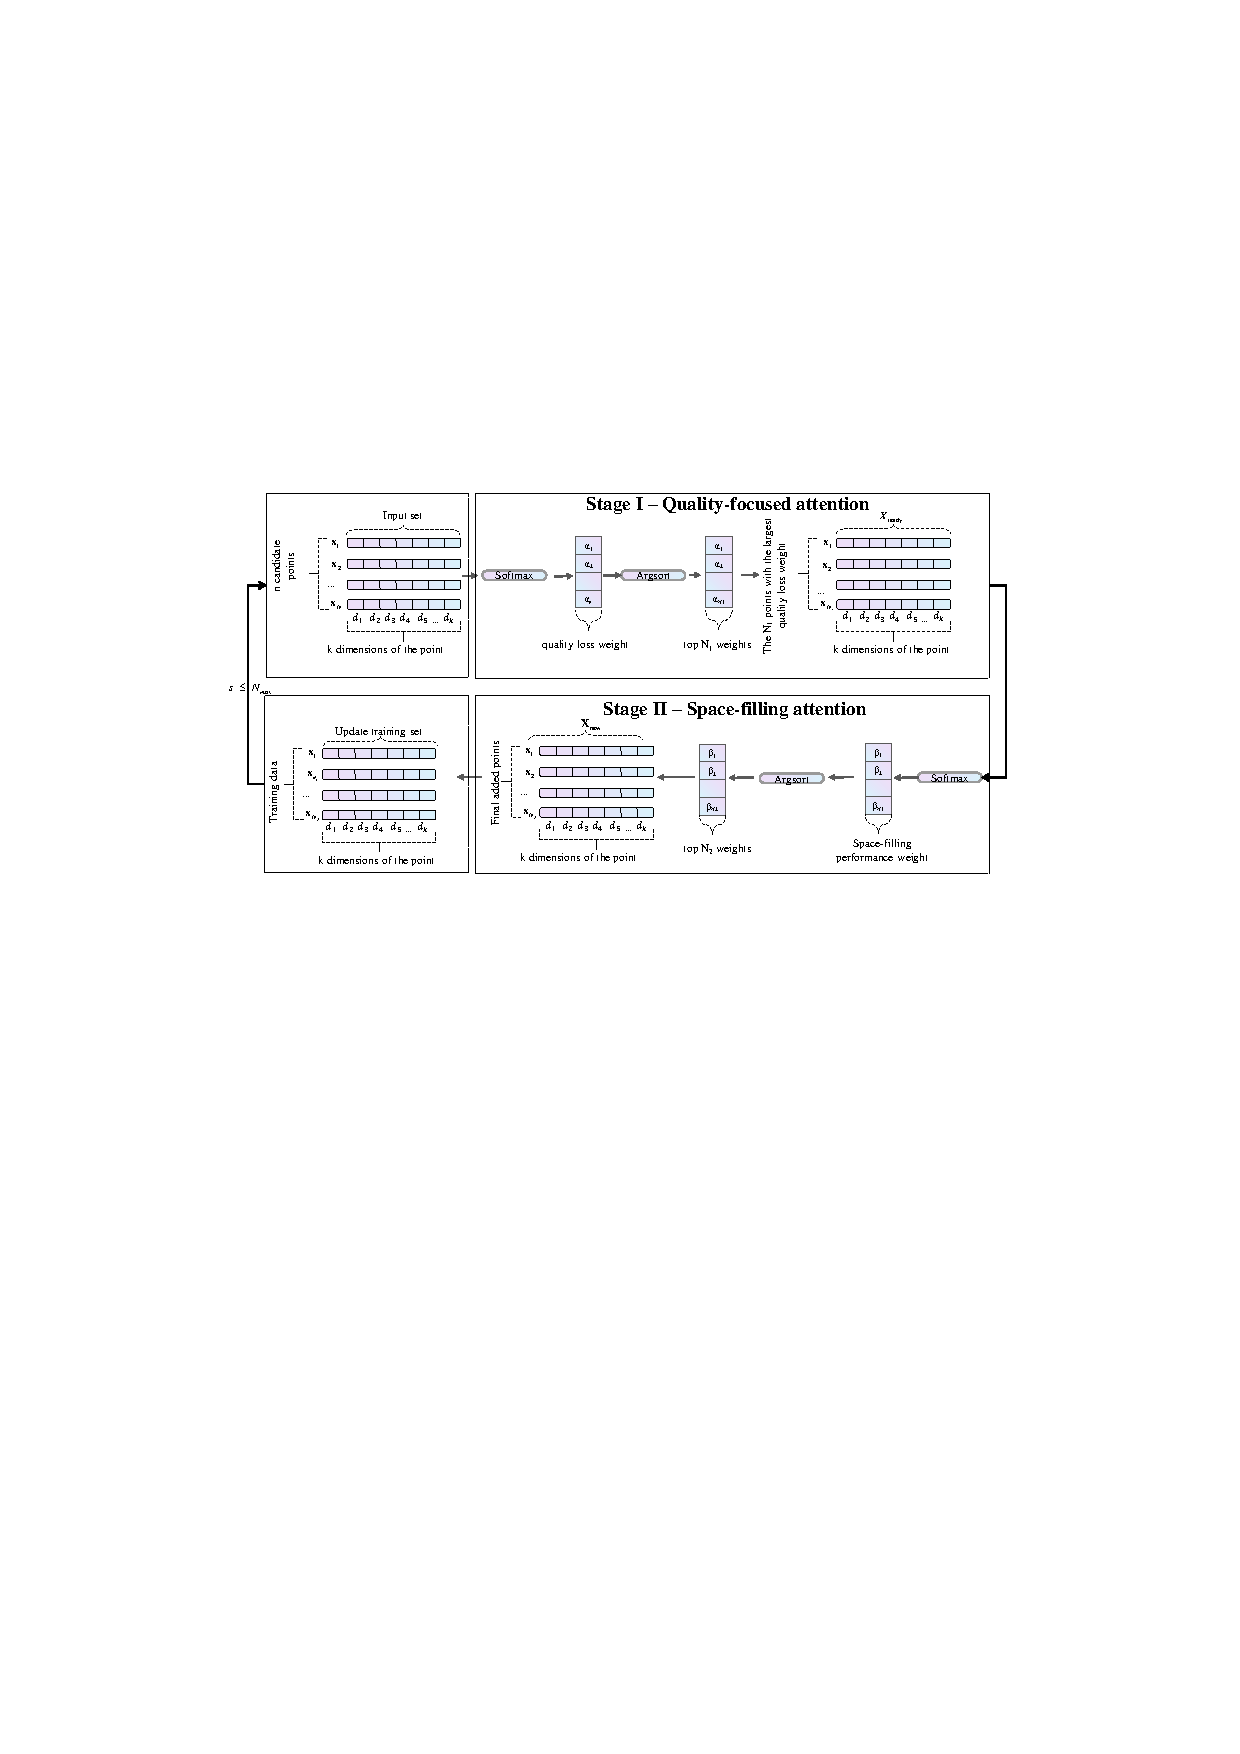
\includegraphics[width=0.9\linewidth]{FIG1.pdf}
	\caption{基于注意力的主动学习 NSGP 建模流程。}
	\label{fig:procedure}
\end{figure}

\subsection{所提稳健优化方法}
本文提出的两阶段注意力主动学习方法用于 NSGP 建模与参数优化，其流程如图~2 所示。
\begin{description}
	\item[步骤 1：] 使用初始训练样本拟合初始 NSGP 模型。
	\item[步骤 2：] 利用式~(17)--(18) 给出的初始模型输出构造质量损失函数和空间距离函数。
	\item[步骤 3：] 结合步骤 2 中的两个指标，构建两阶段注意力采集函数。
	\item[步骤 4：] 应用算法~1 所述主动学习过程选择新的设计点。
	\item[步骤 5：] 更新训练数据集和 NSGP 模型，获得预测响应均值与方差。
	\item[步骤 6：] 基于步骤 5 的预测均值与方差，将质量损失函数构造为稳健优化目标。
	\item[步骤 7：] 使用 genetic algorithm（GA）在输入变量可行域内搜索全局最优，从而确定最优参数设置。
\end{description}
\begin{figure}[h!]
	\centering
	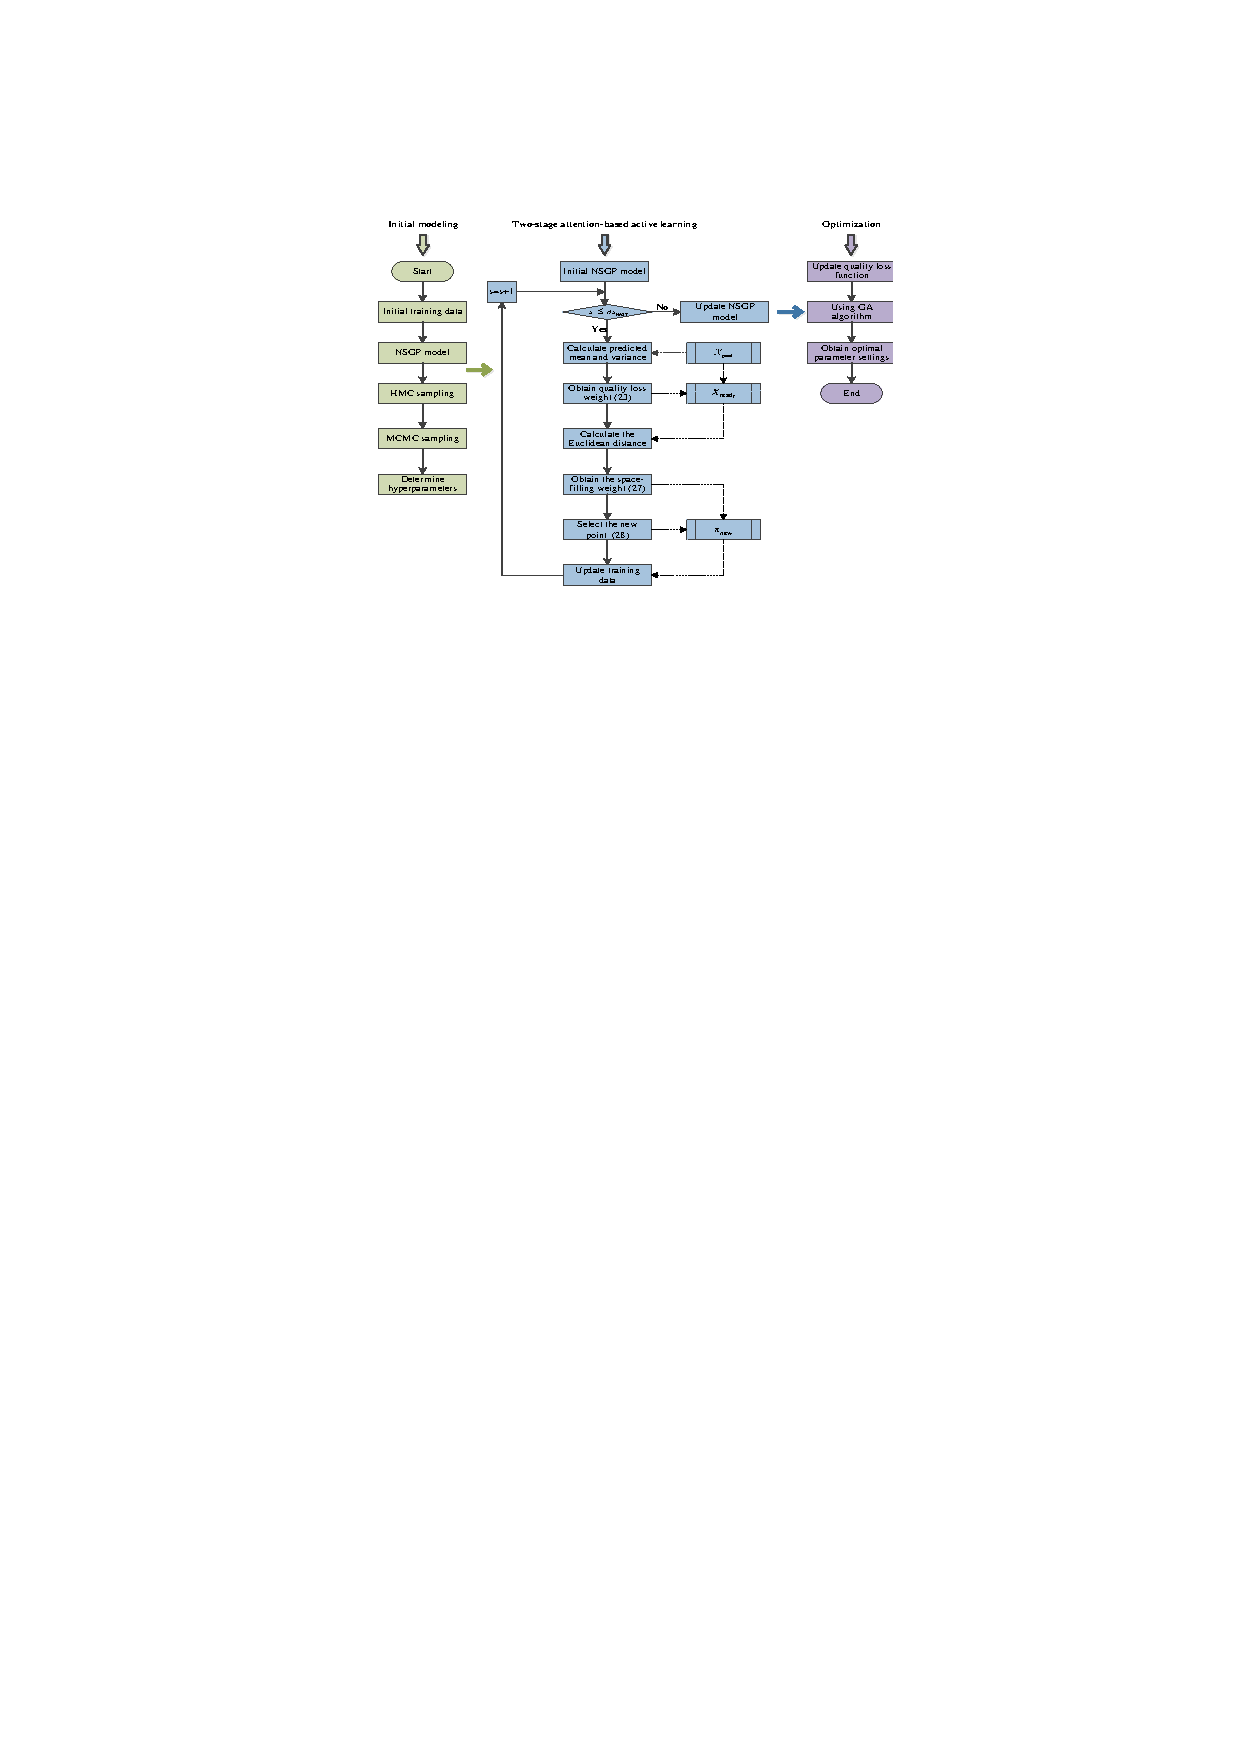
\includegraphics[width=0.8\linewidth]{FIG2.pdf}
	\caption{所提 NSGP 建模与参数优化方法流程图。}
	\label{fig:fig2}
\end{figure}


\section{案例研究}
\subsection{二维数值算例}
本节采用一个二维测试函数验证所提方法的有效性。该函数为分段定义的响应面，在二维输入空间中呈现明显非平稳性。$f(x_{1}, x_{2})$ 的数学表达式为：
\begin{equation}
	f({x_1},{x_2}) = \left\{ {\begin{array}{*{20}{l}}
			{(2 + 0.5{x_2})\sin ({x_1}) + x_2^2,}&{{\rm{if  }}{x_1} > 0},\\
			{x_1^2 + x_2^2 + \left( {8 - (x_1^2 + x_2^2)} \right)\left( {1 - {e^{ - x_1^2}}} \right)},&{{\rm{if  }}{x_1} \le 0},
	\end{array}} \right.
\end{equation}
其中 $(x_{1}, x_{2}) \in [-2, 2]^{2}$。当 $x_{1} > 0$ 时，函数沿 $x_{1}$ 方向呈周期振荡；当 $x_{1} \le 0$ 时，函数呈圆对称且较平滑的响应。该行为反映了显著的非平稳性和结构不连续性。为进一步评估模型在目标区域内的局部预测性能，本文为该测试函数定义特定目标值 $f^{*}$。围绕该目标值，感兴趣区域 ${\mathcal{R}}^{t}$ 定义为满足以下条件的输入点集合：
\begin{equation}
	{{\cal R}^t} = \left\{ {({x_1},{x_2}) \in {\cal X}\left| {\left| {f({x_1},{x_2}) - {f^*}} \right| < t} \right.} \right\},
\end{equation}
其中 $t > 0$ 为预设阈值。集合 ${\mathcal{R}}^{t}$ 可视为设计空间中的潜在最优子区域，其预测精度对稳健优化至关重要。本文将目标值设为 $f^{*} = 1.5$，有意避开极值点，以避免极值行为造成误导。为量化预测值与真实值之间的差异，采用 root mean square error（RMSE）作为性能指标，定义如下：
\begin{equation}
	{\rm{RMSE}} = \sqrt {\frac{1}{n}\sum\limits_{i = 1}^n {{{\left( {\hat f(x_1^i,x_2^i) - f(x_1^i,x_2^i)} \right)}^2}} } ,
\end{equation}
其中，$\hat{f}(x_{1}^{i}, x_{2}^{i})$ 表示模型预测值，$f(x_{1}^{i}, x_{2}^{i})$ 为真实值，$n$ 为测试样本总数。

在该实验中，首先采用 Latin hypercube sampling（LHS）生成 $20$ 个初始设计样本，并用于拟合初始 NSGP 模型。随后，使用所提两阶段注意力主动学习方法选取额外样本，最终得到 $40$--$100$ 个设计点。\reviewadd{为进行直接比较，本文选取两类共八种基准方法：（1）经典实验设计方法，包括 G-optimality（GO）\citep{Omwando2024}、D-optimality（DO）\citep{Lichota2016}、LHS \citep{Guo2023} 和 centroidal Voronoi tessellations（CVT）\citep{Vassiliades2018}；（2）现代主动学习与 Bayesian optimization 采集函数，包括 Expected Improvement（EI）\citep{Jones1998}、Integrated Mean Squared Error reduction（IMSE）\citep{Sacks1989} 和 Upper Confidence Bound（UCB）\citep{Srinivas2010}。}{R1-2, R2-4}所有方法使用相同总样本数。不同方法在二维设计空间中获得的 $40$ 个设计点空间分布如图~3 所示。
\begin{figure}[h]
	\centering
	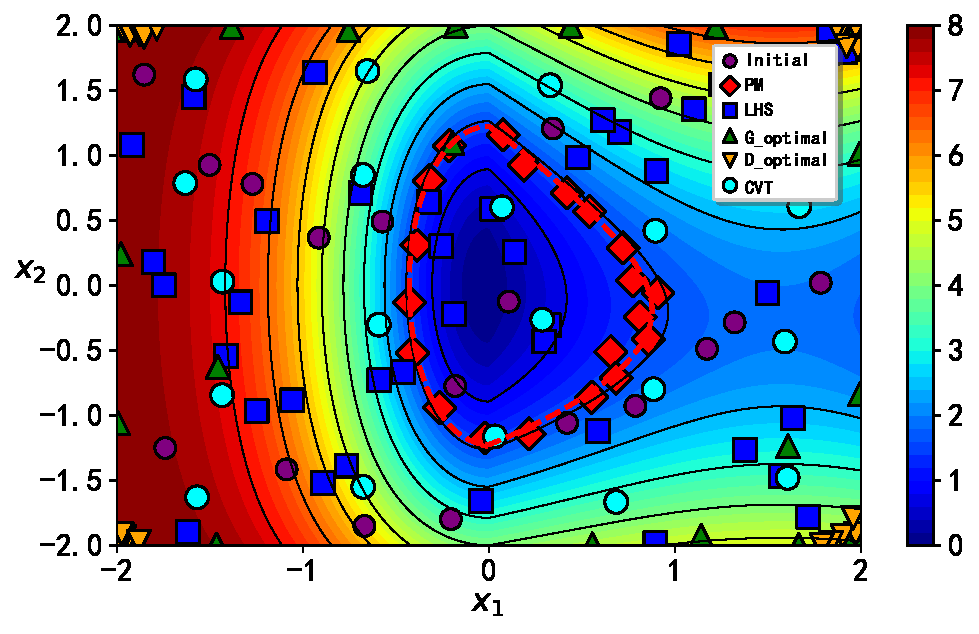
\includegraphics[width=0.7\linewidth]{FIG3.pdf}
	\caption{不同方法获得的 40 个设计点空间分布。}
	\label{fig:design-points}
\end{figure}

图 3 中，紫色圆点表示初始设计点，红色菱形表示所提主动学习方法选取的点，红色虚线表示目标值 $1.5$ 对应的等值线。可以看出，所提方法（PM）选取的设计点主要集中于目标值等值线附近。这说明算法倾向于将实验点分配到潜在最优区域。同时，靠近目标等值线的设计点具有较均匀的空间分布，没有明显重叠或聚集，体现了所提主动学习方法良好的空间填充能力。

为进一步展示所提方法的预测精度优势，本文评估潜在最优区域内的 RMSE 值（RMSE in the target region）和整体响应面上的 RMSE 值（RMSE over the full surface），并在不同总训练样本数（40--100）以及不同新增设计点数（10 和 20）下进行比较。对每种方法，RMSE 计算重复 30 次，以保证比较结果可靠。\reviewadd{结果汇总于表~\ref{tab:rmse_target_10}--\ref{tab:rmse_all_20} 和图~\ref{fig:rmse_combined}。其中，表~\ref{tab:rmse_target_10} 和表~\ref{tab:rmse_target_20} 分别报告新增 10 个和 20 个主动学习设计点时的目标区域 RMSE 及 PM 改善率；表~\ref{tab:rmse_all_10} 和表~\ref{tab:rmse_all_20} 报告对应的整体响应面 RMSE 及 PM 损失率。整体响应面的 PM 损失率定义为 $(\mathrm{RMSE}_{\mathrm{PM}}-\mathrm{RMSE}_{\mathrm{baseline}})/\mathrm{RMSE}_{\mathrm{baseline}}$，正值表示 PM 在整体响应面预测上付出的全局精度损失。}{R1-3}其他统计量（中位数、最大值、最小值、Q1、Q3）见附录~A。

% --- 表1--表4: 由脚本生成的二维 RMSE 对比表 ---
\begin{table}[h!]
\centering
\caption{\reviewadd{新增 10 个主动学习点时目标区域 RMSE 及 PM 改善率。}{R1-2, R2-4}}
\label{tab:rmse_target_10}
\begingroup\color{red}
\resizebox{\linewidth}{!}{%
\begin{tabular}{c rrrrrrrr c rrrrrrrr}
\toprule
\multirow{2}{*}{Number} & \multicolumn{8}{c}{RMSE (Mean)} & & \multicolumn{8}{c}{RMSE (Median)} \\
\cmidrule(lr){2-9} \cmidrule(lr){11-18}
& DO & EI & GO & IMSE & CVT & LHS & PM & UCB & & DO & EI & GO & IMSE & CVT & LHS & PM & UCB \\
\midrule
40 & 0.0919 & 0.1147 & 0.0894 & 0.0783 & 0.0651 & 0.0780 & 0.0562 & 0.1216 &  & 0.0854 & 0.1044 & 0.0823 & 0.0762 & 0.0639 & 0.0675 & 0.0503 & 0.0995 \\
50 & 0.0621 & 0.0633 & 0.0650 & 0.0593 & 0.0560 & 0.0565 & 0.0386 & 0.0626 &  & 0.0621 & 0.0599 & 0.0663 & 0.0589 & 0.0586 & 0.0539 & 0.0382 & 0.0582 \\
60 & 0.0514 & 0.0487 & 0.0540 & 0.0443 & 0.0532 & 0.0451 & 0.0369 & 0.0486 &  & 0.0487 & 0.0472 & 0.0548 & 0.0450 & 0.0430 & 0.0448 & 0.0362 & 0.0470 \\
70 & 0.0427 & 0.0406 & 0.0442 & 0.0399 & 0.0365 & 0.0392 & 0.0317 & 0.0408 &  & 0.0430 & 0.0409 & 0.0419 & 0.0414 & 0.0357 & 0.0349 & 0.0325 & 0.0407 \\
80 & 0.0369 & 0.0360 & 0.0416 & 0.0355 & 0.0333 & 0.0330 & 0.0246 & 0.0363 &  & 0.0365 & 0.0362 & 0.0390 & 0.0353 & 0.0309 & 0.0320 & 0.0241 & 0.0362 \\
90 & 0.0308 & 0.0279 & 0.0323 & 0.0280 & 0.0296 & 0.0261 & 0.0216 & 0.0289 &  & 0.0288 & 0.0283 & 0.0317 & 0.0282 & 0.0264 & 0.0266 & 0.0204 & 0.0285 \\
100 & 0.0225 & 0.0277 & 0.0249 & 0.0248 & 0.0252 & 0.0238 & 0.0181 & 0.0271 &  & 0.0228 & 0.0251 & 0.0250 & 0.0242 & 0.0232 & 0.0228 & 0.0192 & 0.0248 \\
\midrule
\multirow{2}{*}{Number} & \multicolumn{8}{c}{PM Improvement (Mean, \%)} & & \multicolumn{8}{c}{PM Improvement (Median, \%)} \\
\cmidrule(lr){2-9} \cmidrule(lr){11-18}
& DO & EI & GO & IMSE & CVT & LHS & PM & UCB & & DO & EI & GO & IMSE & CVT & LHS & PM & UCB \\
\midrule
40 & 38.81\% & 51.00\% & 37.10\% & 28.17\% & 13.64\% & 27.93\% & -- & 53.78\% &  & 41.05\% & 51.77\% & 38.87\% & 33.92\% & 21.27\% & 25.43\% & -- & 49.41\% \\
50 & 37.92\% & 39.07\% & 40.64\% & 34.97\% & 31.15\% & 31.70\% & -- & 38.38\% &  & 38.44\% & 36.24\% & 42.39\% & 35.17\% & 34.80\% & 29.13\% & -- & 34.32\% \\
60 & 28.20\% & 24.29\% & 31.65\% & 16.76\% & 30.61\% & 18.27\% & -- & 24.05\% &  & 25.57\% & 23.30\% & 33.92\% & 19.58\% & 15.79\% & 19.15\% & -- & 22.95\% \\
70 & 25.72\% & 21.83\% & 28.16\% & 20.41\% & 13.13\% & 18.99\% & -- & 22.20\% &  & 24.38\% & 20.46\% & 22.46\% & 21.41\% & 8.85\% & 6.91\% & -- & 20.07\% \\
80 & 33.30\% & 31.54\% & 40.76\% & 30.57\% & 25.94\% & 25.42\% & -- & 32.15\% &  & 33.84\% & 33.35\% & 38.11\% & 31.72\% & 21.91\% & 24.67\% & -- & 33.47\% \\
90 & 29.89\% & 22.61\% & 33.22\% & 22.85\% & 27.09\% & 17.34\% & -- & 25.33\% &  & 29.15\% & 27.89\% & 35.59\% & 27.43\% & 22.56\% & 23.29\% & -- & 28.31\% \\
100 & 19.42\% & 34.51\% & 27.32\% & 26.89\% & 28.10\% & 23.70\% & -- & 33.01\% &  & 16.06\% & 23.75\% & 23.38\% & 20.71\% & 17.42\% & 15.97\% & -- & 22.53\% \\
\bottomrule
\end{tabular}%
}
\endgroup
\end{table}

\begin{table}[h!]
\centering
\caption{\reviewadd{新增 10 个主动学习点时整体响应面 RMSE 及 PM 损失率。}{R1-3}}
\label{tab:rmse_all_10}
\begingroup\color{red}
\resizebox{\linewidth}{!}{%
\begin{tabular}{c rrrrrrrr c rrrrrrrr}
\toprule
\multirow{2}{*}{Number} & \multicolumn{8}{c}{RMSE (Mean)} & & \multicolumn{8}{c}{RMSE (Median)} \\
\cmidrule(lr){2-9} \cmidrule(lr){11-18}
& DO & EI & GO & IMSE & CVT & LHS & PM & UCB & & DO & EI & GO & IMSE & CVT & LHS & PM & UCB \\
\midrule
40 & 0.1088 & 0.1787 & 0.0838 & 0.0772 & 0.1088 & 0.1253 & 0.1687 & 0.1883 &  & 0.1053 & 0.1607 & 0.0843 & 0.0754 & 0.1070 & 0.1099 & 0.1537 & 0.1667 \\
50 & 0.0773 & 0.1096 & 0.0552 & 0.0539 & 0.0724 & 0.0792 & 0.1003 & 0.1113 &  & 0.0723 & 0.1008 & 0.0548 & 0.0548 & 0.0679 & 0.0770 & 0.0925 & 0.1047 \\
60 & 0.0589 & 0.0931 & 0.0429 & 0.0412 & 0.0618 & 0.0690 & 0.0963 & 0.0923 &  & 0.0544 & 0.0871 & 0.0427 & 0.0420 & 0.0593 & 0.0591 & 0.0796 & 0.0878 \\
70 & 0.0438 & 0.0622 & 0.0335 & 0.0362 & 0.0501 & 0.0498 & 0.0548 & 0.0629 &  & 0.0438 & 0.0548 & 0.0327 & 0.0361 & 0.0504 & 0.0441 & 0.0542 & 0.0553 \\
80 & 0.0350 & 0.0476 & 0.0301 & 0.0294 & 0.0390 & 0.0388 & 0.0419 & 0.0480 &  & 0.0338 & 0.0450 & 0.0305 & 0.0291 & 0.0417 & 0.0378 & 0.0395 & 0.0450 \\
90 & 0.0290 & 0.0389 & 0.0242 & 0.0231 & 0.0312 & 0.0316 & 0.0351 & 0.0396 &  & 0.0280 & 0.0351 & 0.0237 & 0.0233 & 0.0292 & 0.0304 & 0.0292 & 0.0348 \\
100 & 0.0222 & 0.0295 & 0.0200 & 0.0214 & 0.0248 & 0.0261 & 0.0338 & 0.0290 &  & 0.0219 & 0.0273 & 0.0195 & 0.0214 & 0.0244 & 0.0252 & 0.0316 & 0.0281 \\
\midrule
\multirow{2}{*}{Number} & \multicolumn{8}{c}{PM Loss Rate (Mean, \%)} & & \multicolumn{8}{c}{PM Loss Rate (Median, \%)} \\
\cmidrule(lr){2-9} \cmidrule(lr){11-18}
& DO & EI & GO & IMSE & CVT & LHS & PM & UCB & & DO & EI & GO & IMSE & CVT & LHS & PM & UCB \\
\midrule
40 & 55.01\% & -5.59\% & 101.39\% & 118.45\% & 55.09\% & 34.68\% & -- & -10.43\% &  & 45.91\% & -4.36\% & 82.35\% & 103.75\% & 43.65\% & 39.78\% & -- & -7.80\% \\
50 & 29.77\% & -8.51\% & 81.69\% & 85.92\% & 38.50\% & 26.64\% & -- & -9.90\% &  & 27.96\% & -8.25\% & 68.68\% & 68.91\% & 36.27\% & 20.09\% & -- & -11.64\% \\
60 & 63.56\% & 3.40\% & 124.69\% & 133.74\% & 55.91\% & 39.60\% & -- & 4.33\% &  & 46.49\% & -8.57\% & 86.31\% & 89.66\% & 34.32\% & 34.64\% & -- & -9.27\% \\
70 & 25.10\% & -12.00\% & 63.36\% & 51.39\% & 9.40\% & 10.05\% & -- & -12.95\% &  & 23.86\% & -1.02\% & 65.79\% & 50.05\% & 7.59\% & 22.99\% & -- & -1.92\% \\
80 & 19.57\% & -11.95\% & 39.04\% & 42.36\% & 7.49\% & 7.79\% & -- & -12.77\% &  & 17.01\% & -12.16\% & 29.47\% & 35.77\% & -5.33\% & 4.51\% & -- & -12.21\% \\
90 & 21.00\% & -9.68\% & 45.17\% & 51.85\% & 12.54\% & 11.06\% & -- & -11.35\% &  & 4.15\% & -16.79\% & 23.33\% & 25.46\% & -0.14\% & -3.94\% & -- & -16.19\% \\
100 & 52.37\% & 14.53\% & 69.10\% & 58.41\% & 36.29\% & 29.71\% & -- & 16.66\% &  & 44.03\% & 15.47\% & 61.72\% & 47.81\% & 29.62\% & 25.22\% & -- & 12.31\% \\
\bottomrule
\end{tabular}%
}
\endgroup
\end{table}

\begin{table}[h!]
\centering
\caption{\reviewadd{新增 20 个主动学习点时目标区域 RMSE 及 PM 改善率。}{R1-2, R2-4}}
\label{tab:rmse_target_20}
\begingroup\color{red}
\resizebox{\linewidth}{!}{%
\begin{tabular}{c rrrrrrrr c rrrrrrrr}
\toprule
\multirow{2}{*}{Number} & \multicolumn{8}{c}{RMSE (Mean)} & & \multicolumn{8}{c}{RMSE (Median)} \\
\cmidrule(lr){2-9} \cmidrule(lr){11-18}
& DO & EI & GO & IMSE & CVT & LHS & PM & UCB & & DO & EI & GO & IMSE & CVT & LHS & PM & UCB \\
\midrule
40 & 0.1517 & 0.1688 & 0.0954 & 0.0824 & 0.0817 & 0.0730 & 0.0540 & 0.2283 &  & 0.1385 & 0.1551 & 0.0890 & 0.0840 & 0.0802 & 0.0644 & 0.0310 & 0.1882 \\
50 & 0.0990 & 0.1056 & 0.0530 & 0.0551 & 0.0719 & 0.0538 & 0.0324 & 0.1319 &  & 0.0954 & 0.0951 & 0.0530 & 0.0550 & 0.0730 & 0.0510 & 0.0249 & 0.1104 \\
60 & 0.0499 & 0.0574 & 0.0481 & 0.0481 & 0.0565 & 0.0396 & 0.0216 & 0.0593 &  & 0.0481 & 0.0483 & 0.0458 & 0.0481 & 0.0562 & 0.0390 & 0.0207 & 0.0472 \\
70 & 0.0453 & 0.0381 & 0.0410 & 0.0371 & 0.0511 & 0.0359 & 0.0235 & 0.0360 &  & 0.0466 & 0.0367 & 0.0422 & 0.0365 & 0.0503 & 0.0356 & 0.0222 & 0.0302 \\
80 & 0.0345 & 0.0384 & 0.0400 & 0.0319 & 0.0419 & 0.0359 & 0.0223 & 0.0349 &  & 0.0367 & 0.0377 & 0.0378 & 0.0330 & 0.0431 & 0.0347 & 0.0205 & 0.0336 \\
90 & 0.0319 & 0.0287 & 0.0298 & 0.0260 & 0.0391 & 0.0263 & 0.0187 & 0.0301 &  & 0.0298 & 0.0295 & 0.0310 & 0.0261 & 0.0377 & 0.0263 & 0.0180 & 0.0281 \\
100 & 0.0281 & 0.0260 & 0.0321 & 0.0230 & 0.0354 & 0.0227 & 0.0173 & 0.0251 &  & 0.0281 & 0.0253 & 0.0328 & 0.0228 & 0.0352 & 0.0230 & 0.0164 & 0.0247 \\
\midrule
\multirow{2}{*}{Number} & \multicolumn{8}{c}{PM Improvement (Mean, \%)} & & \multicolumn{8}{c}{PM Improvement (Median, \%)} \\
\cmidrule(lr){2-9} \cmidrule(lr){11-18}
& DO & EI & GO & IMSE & CVT & LHS & PM & UCB & & DO & EI & GO & IMSE & CVT & LHS & PM & UCB \\
\midrule
40 & 64.38\% & 67.98\% & 43.37\% & 34.43\% & 33.84\% & 25.98\% & -- & 76.33\% &  & 77.63\% & 80.02\% & 65.18\% & 63.11\% & 61.37\% & 51.92\% & -- & 83.53\% \\
50 & 67.24\% & 69.29\% & 38.79\% & 41.16\% & 54.86\% & 39.74\% & -- & 75.40\% &  & 73.86\% & 73.79\% & 52.92\% & 54.64\% & 65.83\% & 51.16\% & -- & 77.43\% \\
60 & 56.67\% & 62.34\% & 55.05\% & 55.06\% & 61.75\% & 45.46\% & -- & 63.53\% &  & 56.98\% & 57.16\% & 54.85\% & 56.96\% & 63.16\% & 46.93\% & -- & 56.15\% \\
70 & 48.23\% & 38.47\% & 42.81\% & 36.71\% & 54.13\% & 34.59\% & -- & 34.79\% &  & 52.42\% & 39.52\% & 47.46\% & 39.15\% & 55.92\% & 37.66\% & -- & 26.44\% \\
80 & 35.45\% & 41.92\% & 44.32\% & 30.00\% & 46.80\% & 37.97\% & -- & 36.18\% &  & 44.16\% & 45.62\% & 45.70\% & 37.76\% & 52.43\% & 40.85\% & -- & 38.90\% \\
90 & 41.36\% & 34.80\% & 37.30\% & 28.00\% & 52.20\% & 28.91\% & -- & 37.81\% &  & 39.58\% & 38.98\% & 41.99\% & 31.07\% & 52.31\% & 31.61\% & -- & 36.03\% \\
100 & 38.54\% & 33.41\% & 46.15\% & 24.75\% & 51.10\% & 23.93\% & -- & 31.11\% &  & 41.49\% & 35.07\% & 49.83\% & 27.77\% & 53.33\% & 28.52\% & -- & 33.43\% \\
\bottomrule
\end{tabular}%
}
\endgroup
\end{table}

\begin{table}[h!]
\centering
\caption{\reviewadd{新增 20 个主动学习点时整体响应面 RMSE 及 PM 损失率。}{R1-3}}
\label{tab:rmse_all_20}
\begingroup\color{red}
\resizebox{\linewidth}{!}{%
\begin{tabular}{c rrrrrrrr c rrrrrrrr}
\toprule
\multirow{2}{*}{Number} & \multicolumn{8}{c}{RMSE (Mean)} & & \multicolumn{8}{c}{RMSE (Median)} \\
\cmidrule(lr){2-9} \cmidrule(lr){11-18}
& DO & EI & GO & IMSE & CVT & LHS & PM & UCB & & DO & EI & GO & IMSE & CVT & LHS & PM & UCB \\
\midrule
40 & 0.1580 & 0.1741 & 0.0873 & 0.0787 & 0.0964 & 0.1121 & 0.3268 & 0.3043 &  & 0.1473 & 0.1522 & 0.0839 & 0.0809 & 0.0943 & 0.0972 & 0.2884 & 0.2707 \\
50 & 0.1207 & 0.1093 & 0.0540 & 0.0527 & 0.0794 & 0.0739 & 0.1537 & 0.2142 &  & 0.1068 & 0.1014 & 0.0549 & 0.0516 & 0.0775 & 0.0745 & 0.1499 & 0.1940 \\
60 & 0.0691 & 0.0844 & 0.0413 & 0.0425 & 0.0560 & 0.0670 & 0.1068 & 0.0971 &  & 0.0608 & 0.0719 & 0.0412 & 0.0417 & 0.0562 & 0.0615 & 0.1073 & 0.0909 \\
70 & 0.0499 & 0.0690 & 0.0349 & 0.0329 & 0.0456 & 0.0508 & 0.0729 & 0.0634 &  & 0.0488 & 0.0644 & 0.0347 & 0.0334 & 0.0445 & 0.0493 & 0.0660 & 0.0549 \\
80 & 0.0378 & 0.0578 & 0.0308 & 0.0274 & 0.0378 & 0.0392 & 0.0571 & 0.0586 &  & 0.0350 & 0.0490 & 0.0301 & 0.0277 & 0.0378 & 0.0391 & 0.0503 & 0.0527 \\
90 & 0.0355 & 0.0401 & 0.0250 & 0.0217 & 0.0301 & 0.0334 & 0.0495 & 0.0427 &  & 0.0332 & 0.0404 & 0.0251 & 0.0222 & 0.0288 & 0.0308 & 0.0410 & 0.0421 \\
100 & 0.0306 & 0.0354 & 0.0215 & 0.0193 & 0.0282 & 0.0287 & 0.0339 & 0.0374 &  & 0.0296 & 0.0317 & 0.0212 & 0.0191 & 0.0289 & 0.0261 & 0.0317 & 0.0324 \\
\midrule
\multirow{2}{*}{Number} & \multicolumn{8}{c}{PM Loss Rate (Mean, \%)} & & \multicolumn{8}{c}{PM Loss Rate (Median, \%)} \\
\cmidrule(lr){2-9} \cmidrule(lr){11-18}
& DO & EI & GO & IMSE & CVT & LHS & PM & UCB & & DO & EI & GO & IMSE & CVT & LHS & PM & UCB \\
\midrule
40 & 106.81\% & 87.72\% & 274.23\% & 315.09\% & 238.90\% & 191.50\% & -- & 7.40\% &  & 95.78\% & 89.52\% & 243.89\% & 256.69\% & 205.87\% & 196.62\% & -- & 6.56\% \\
50 & 27.33\% & 40.59\% & 184.42\% & 191.52\% & 93.57\% & 107.94\% & -- & -28.25\% &  & 40.37\% & 47.78\% & 172.95\% & 190.14\% & 93.33\% & 101.06\% & -- & -22.75\% \\
60 & 54.42\% & 26.47\% & 158.81\% & 151.48\% & 90.74\% & 59.48\% & -- & 9.95\% &  & 76.46\% & 49.37\% & 160.37\% & 157.45\% & 90.99\% & 74.50\% & -- & 18.13\% \\
70 & 46.13\% & 5.56\% & 108.89\% & 121.62\% & 59.74\% & 43.38\% & -- & 15.00\% &  & 35.42\% & 2.61\% & 90.25\% & 97.93\% & 48.41\% & 34.03\% & -- & 20.22\% \\
80 & 51.27\% & -1.15\% & 85.42\% & 108.34\% & 51.27\% & 45.61\% & -- & -2.45\% &  & 43.75\% & 2.58\% & 66.93\% & 81.62\% & 33.01\% & 28.52\% & -- & -4.63\% \\
90 & 39.52\% & 23.43\% & 97.89\% & 127.99\% & 64.16\% & 48.21\% & -- & 15.75\% &  & 23.52\% & 1.69\% & 63.38\% & 84.72\% & 42.42\% & 33.23\% & -- & -2.49\% \\
100 & 10.82\% & -4.01\% & 57.91\% & 75.64\% & 20.43\% & 18.15\% & -- & -9.30\% &  & 6.96\% & 0.01\% & 49.39\% & 65.73\% & 9.64\% & 21.26\% & -- & -2.31\% \\
\bottomrule
\end{tabular}%
}
\endgroup
\end{table}


% --- 图4: 新 RMSE 对比图 (来自 sub/2d/) ---
\begin{figure}[h!]
	\centering
	\subfigure[\reviewadd{10 个主动学习点，目标区域。}{R1-2, R2-4}]{%
		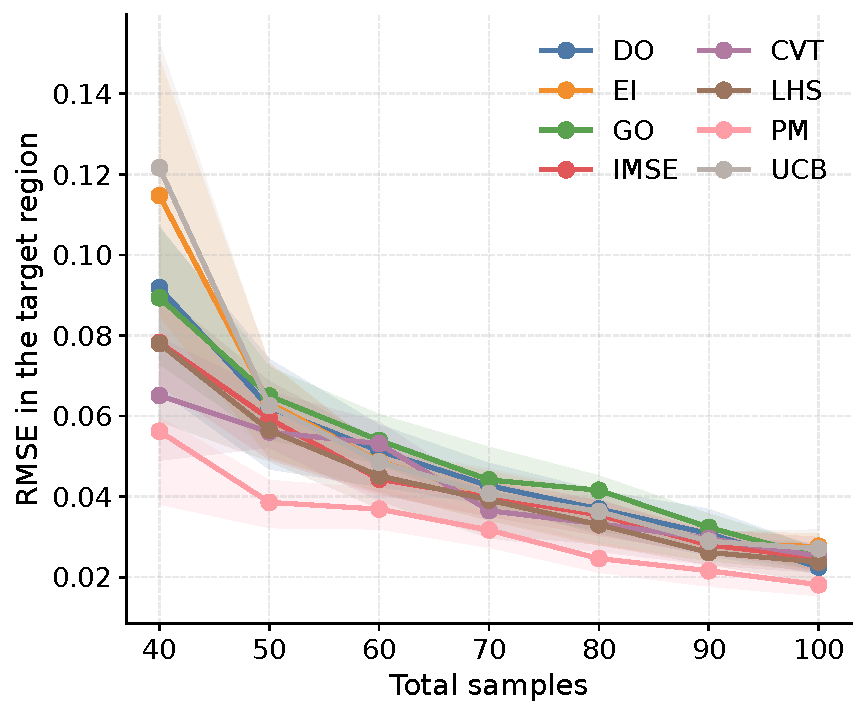
\includegraphics[width=0.48\linewidth]{sub/2d/2d_target_10.pdf}}\hspace{10pt}
	\subfigure[\reviewadd{20 个主动学习点，目标区域。}{R1-2, R2-4}]{%
		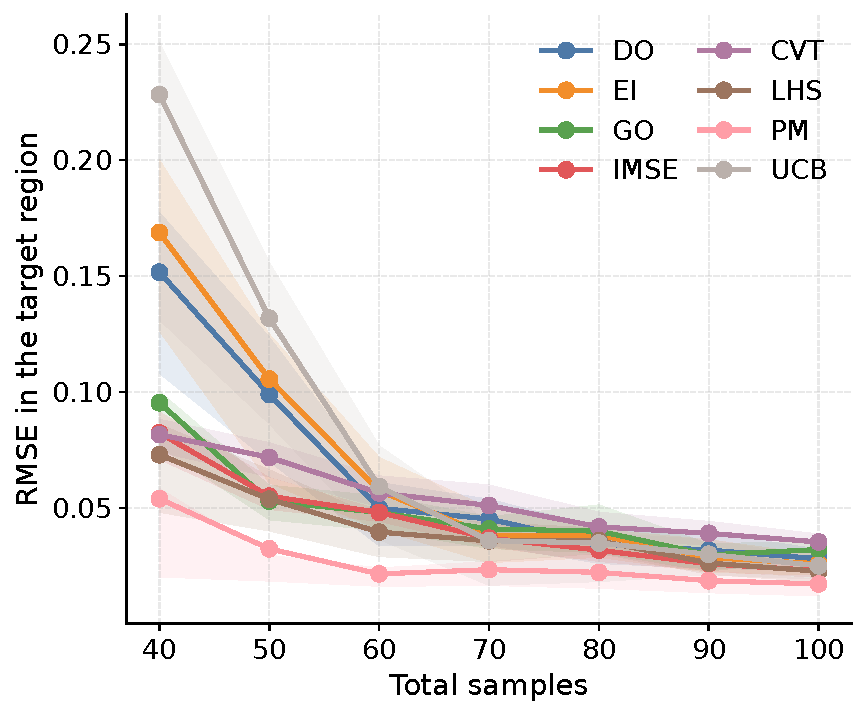
\includegraphics[width=0.48\linewidth]{sub/2d/2d_target_20.pdf}}
	
	\subfigure[\reviewadd{10 个主动学习点，整体响应面。}{R1-3}]{%
		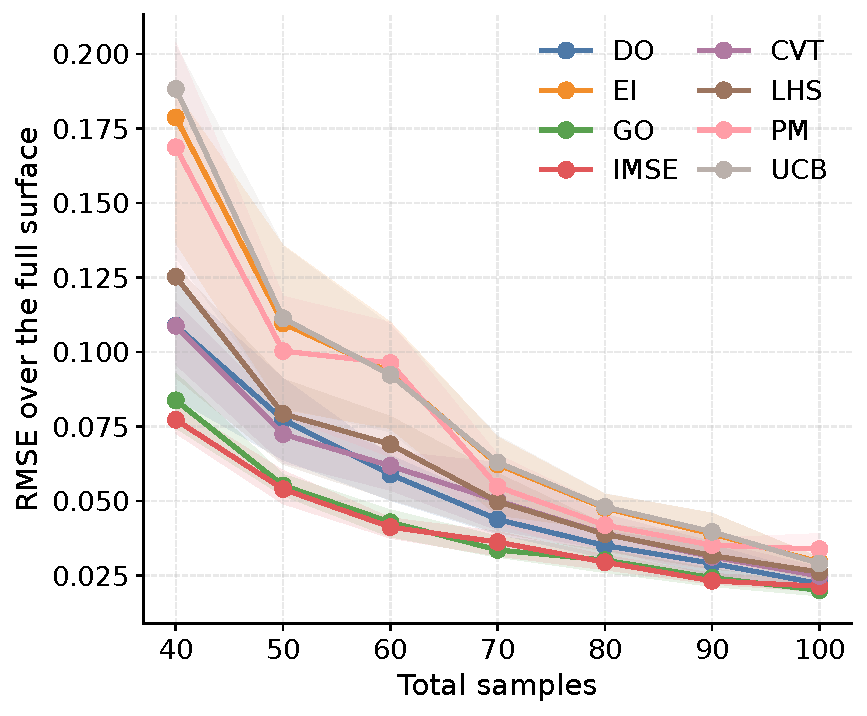
\includegraphics[width=0.48\linewidth]{sub/2d/2d_overall_10.pdf}}\hspace{10pt}
	\subfigure[\reviewadd{20 个主动学习点，整体响应面。}{R1-3}]{%
		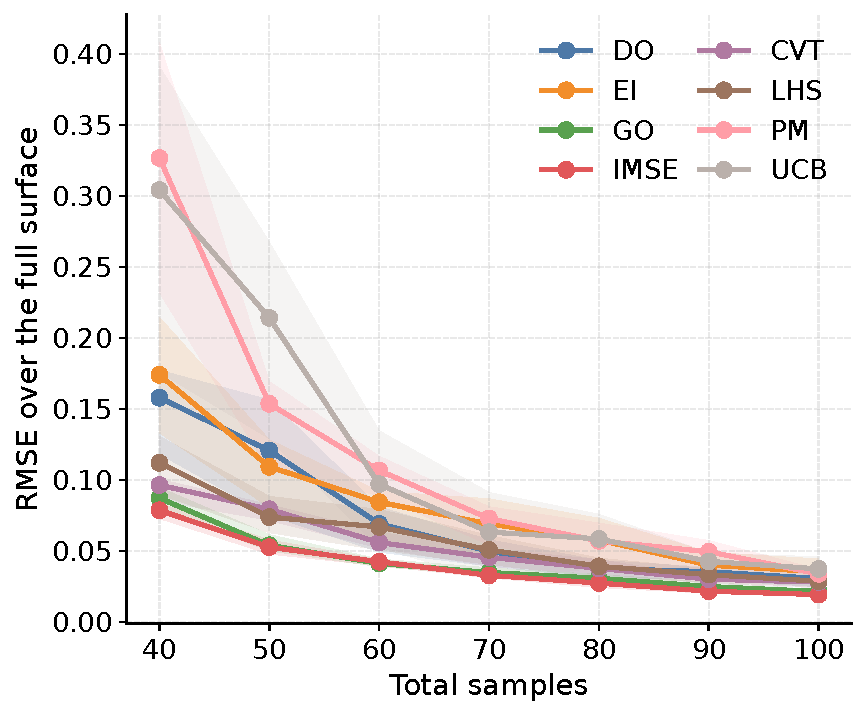
\includegraphics[width=0.48\linewidth]{sub/2d/2d_overall_20.pdf}}
	
	\caption{\reviewadd{不同主动学习设计点数量下的 RMSE 比较（含 EI、UCB、IMSE 基准）：(a)--(b) 潜在最优子区域；(c)--(d) 整体响应面。}{R1-2, R1-3, R2-4}}
	\label{fig:rmse_combined}
\end{figure}

\reviewadd{由表~\ref{tab:rmse_target_10} 可见，当新增 10 个主动学习设计点时，PM 方法在所有训练样本规模下均取得最低目标区域 RMSE。总样本数为 40 时，PM 的目标区域 RMSE 为 0.0562，低于次优 CVT（0.0651），并分别比 EI、IMSE 和 UCB 低 51.00\%、28.22\% 和 53.78\%。当总样本数增加至 100 时，PM 的目标区域 RMSE 进一步降至 0.0181，仍优于所有经典设计方法和现代主动学习基线。}{R1-2, R2-4}

\reviewadd{由表~\ref{tab:rmse_target_20} 可见，当新增 20 个主动学习设计点时，PM 方法同样在全部样本规模下保持最低目标区域 RMSE，且在小样本阶段优势更明显。总样本数为 40 时，PM 的目标区域 RMSE 为 0.0540，分别比 LHS、DO、EI、IMSE 和 UCB 低 26.03\%、64.40\%、68.01\%、34.47\% 和 76.34\%。总样本数为 100 时，PM 的目标区域 RMSE 为 0.0173，仍为所有方法中的最低值。}{R1-2, R2-4}

\reviewadd{表~\ref{tab:rmse_all_10} 和表~\ref{tab:rmse_all_20} 表明，PM 方法的整体响应面 RMSE 在部分样本规模下高于 GO、IMSE 等偏全局探索的方法，对应的 PM 损失率为正。这一现象与方法设计目标一致：PM 将新增设计点优先分配到潜在最优区域，以提升稳健优化所依赖的局部建模精度。以新增 10 个主动学习点且总样本数为 100 的情形为例，PM 相较 DO 的目标区域 RMSE 降低 19.56\%，而整体 RMSE 由 0.0222 增至 0.0338，对应整体响应面损失率为 52.37\%。该结果说明，PM 以可量化的全局精度损失换取了更明显的目标区域精度提升，符合稳健参数设计对潜在最优区域建模精度的要求。}{R1-3}

\reviewadd{为进一步验证两阶段注意力机制各组成部分的作用，本文在二维测试函数上开展消融实验，比较以下七种变体：（1）PM (full)，完整的两阶段 softmax 加权方法；（2）QL only，仅使用第一阶段质量损失准则；（3）MDSF only，仅使用第二阶段 maximin 空间填充准则；（4）Two-stage (no softmax)，保留两阶段结构但去除 softmax 归一化；（5--7）Linear ($\lambda=0.25,0.50,0.75$)，将质量损失与空间距离线性加权，$\lambda$ 为质量损失权重。所有变体使用相同的 20 个初始 LHS 样本和 20 个主动学习新增样本，重复 30 次。结果如图~\ref{fig:ablation_box} 和图~\ref{fig:ablation_vs_n} 所示。}{R1-1, R2-1}

\begin{figure}[h!]
	\centering
	\subfigure[\reviewadd{目标区域 RMSE。}{R1-1, R2-1}]{%
		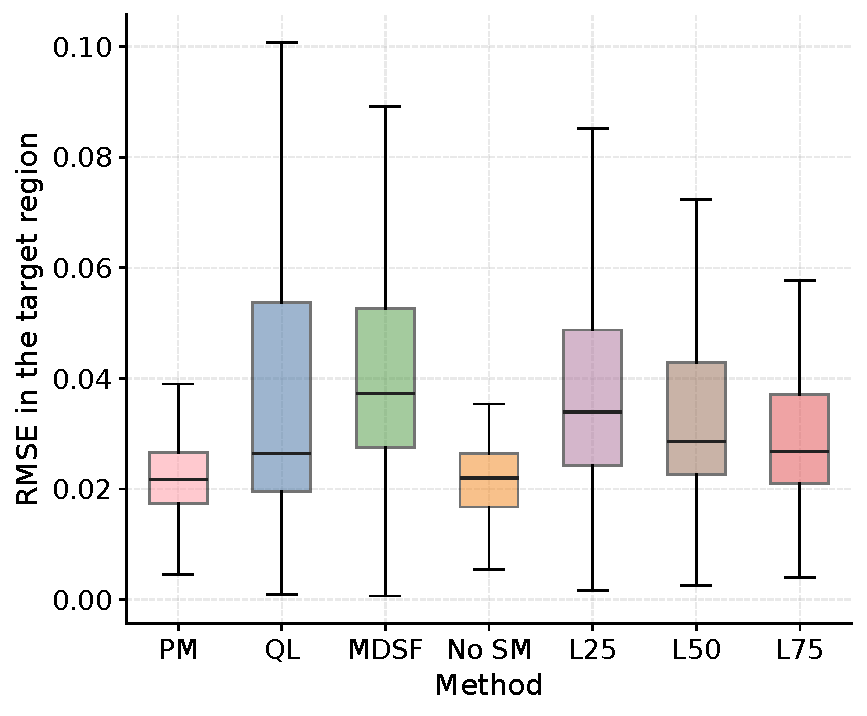
\includegraphics[width=0.48\linewidth]{sub/2d/2d_ablation_rmse_target.pdf}}
	\hfill
	\subfigure[\reviewadd{整体 RMSE。}{R1-1, R2-1}]{%
		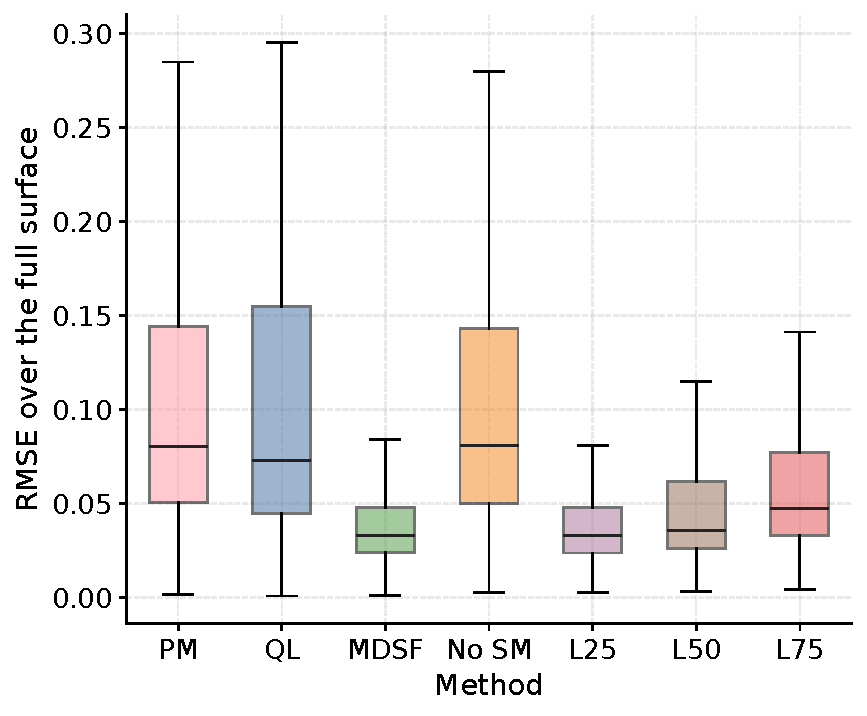
\includegraphics[width=0.48\linewidth]{sub/2d/2d_ablation_rmse_all.pdf}}
	\caption{\reviewadd{消融实验结果：不同变体的 RMSE 分布。}{R1-1, R2-1}}
	\label{fig:ablation_box}
\end{figure}

\begin{figure}[h!]
	\centering
	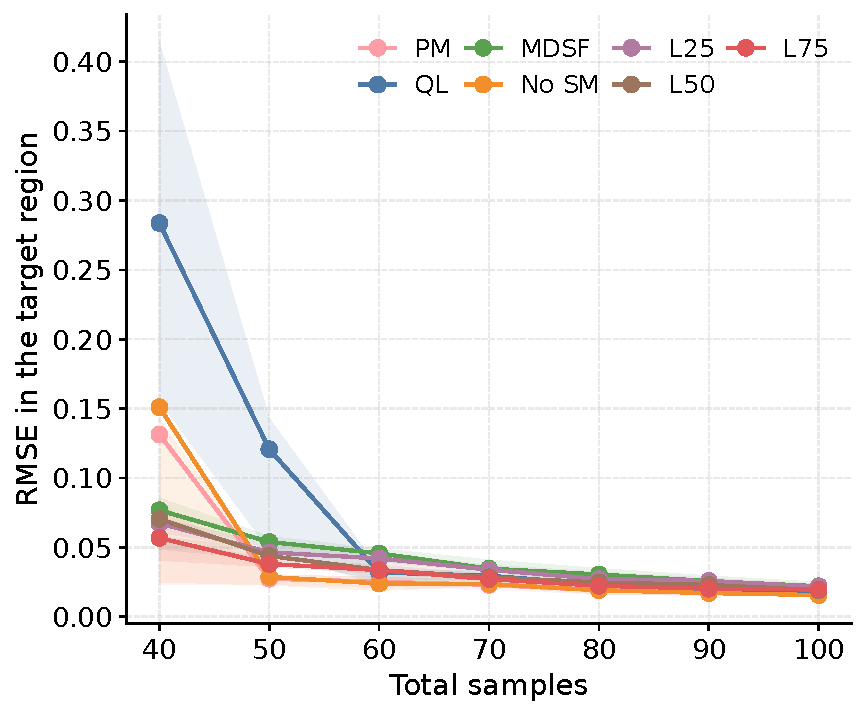
\includegraphics[width=0.48\linewidth]{sub/2d/2d_ablation_rmse_target_vs_n.pdf}
	\caption{\reviewadd{消融实验：目标区域 RMSE 随训练样本总量的变化趋势。}{R1-1, R2-1}}
	\label{fig:ablation_vs_n}
\end{figure}

\reviewadd{消融结果显示，仅使用质量损失的 QL only 变体目标区域 RMSE 均值为 0.0752，约为 PM (full) 的 2.03 倍，说明缺少空间约束时样本易集中于局部区域；仅使用空间填充的 MDSF only 变体整体 RMSE 较低，但目标区域 RMSE 均值升至 0.0413，表明缺少目标引导会削弱潜在最优区域建模。Two-stage (no softmax) 与 PM (full) 接近，但 PM (full) 在目标区域 RMSE 中位数上更低（0.0217 vs. 0.0220），说明 softmax 归一化有助于平滑权重分布并减少硬排序带来的选择波动。线性加权变体在部分样本规模下取得较低目标区域 RMSE，但需要预先设定 $\lambda$，且整体 RMSE 随 $\lambda$ 增大而上升。综合来看，两阶段结构、目标导向质量损失、空间填充约束和 softmax 加权共同构成了 PM 方法稳定发挥作用的关键。}{R1-1, R2-1, R2-3}

\reviewadd{为评估所提方法对采样目标值 $T$ 的敏感性，本文在二维测试函数上选取 $T \in \{0.0, 1.2, 1.3, 1.5, 1.6, 1.7\}$ 作为主动学习引导目标，并始终以 $T=1.5$ 作为评估基准。图~\ref{fig:sensitivity_rmse} 展示了不同采样目标值下目标区域 RMSE 随训练样本总量的变化。}{R2-2}

\begin{figure}[h!]
	\centering
	\subfigure[\reviewadd{目标区域 RMSE 随样本量变化。}{R2-2}]{%
		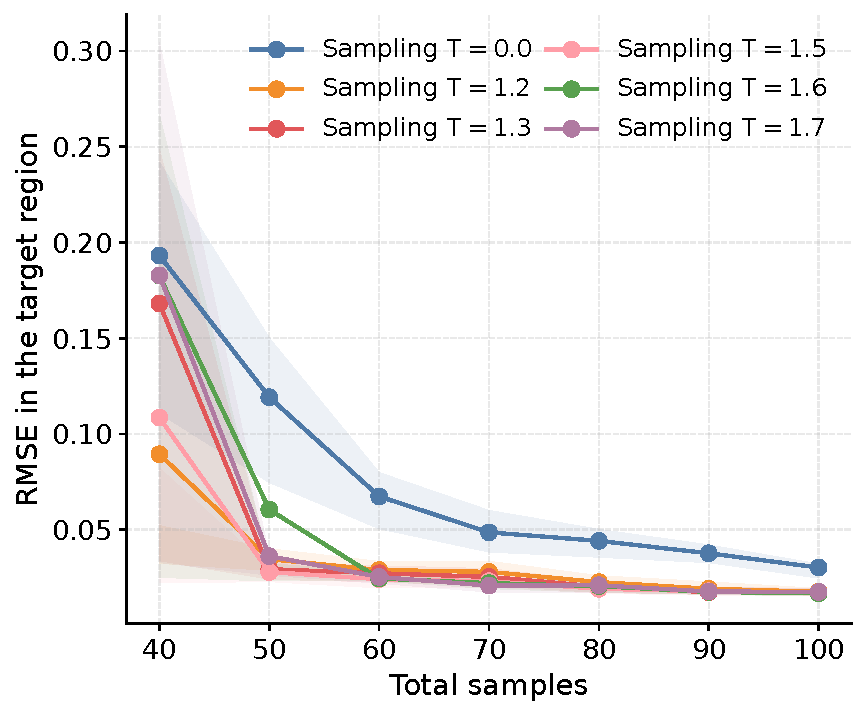
\includegraphics[width=0.48\linewidth]{sub/2d/2d_sensitivity_rmse_target.pdf}}
	\hfill
	\subfigure[\reviewadd{$n=100$ 时不同 $T$ 的对比。}{R2-2}]{%
		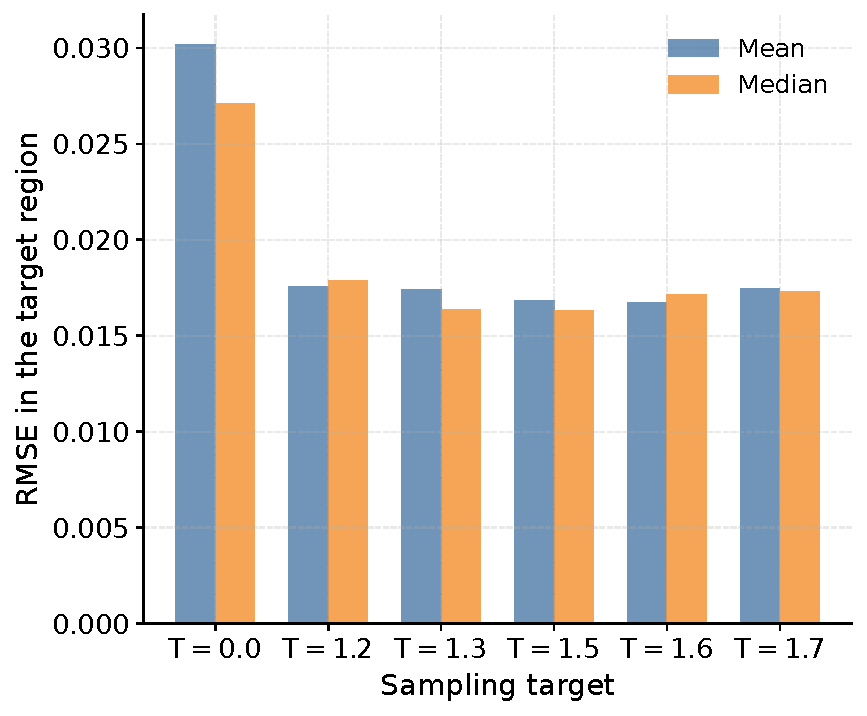
\includegraphics[width=0.48\linewidth]{sub/2d/2d_sensitivity_bar.pdf}}
	\caption{\reviewadd{目标值敏感性分析：不同采样目标值 $T$ 下 PM 方法的目标区域 RMSE。}{R2-2}}
	\label{fig:sensitivity_rmse}
\end{figure}

\reviewadd{结果表明，当采样目标值接近真实评估目标 $1.5$ 时（$T=1.2,1.3,1.5,1.6,1.7$），PM 方法对目标值设定具有较好稳健性。总样本数为 100 时，上述五个采样目标对应的目标区域 RMSE 均值保持在 0.0167--0.0176 之间，差异很小；所有样本规模合并后，其目标区域 RMSE 均值也保持在 0.0339--0.0492 范围内。当采样目标严重偏离评估目标（$T=0.0$）时，目标区域 RMSE 明显升高，合并均值达到 0.0772。该结果说明，实际应用中只要目标值设定不存在明显偏移，PM 方法即可保持稳定的目标区域预测性能；若目标值严重偏离真实质量目标，则采样将被引导至不相关区域，性能会相应下降。}{R2-2}

\reviewadd{\subsection{锂电池荷电状态预测}
本节采用 \cite{Mustafa2024} 提出的锂电池荷电状态（SoC）预测案例评价所提方法性能。在电池放电的不同阶段，SoC 对电流和电压表现出明显不同的响应速率，体现出典型非平稳行为。该案例以 18650 型锂离子电池为研究对象，输出变量为 SoC（\%）。SoC 定义为当前电量相对于电池总容量的百分比，取值范围为 $y \in [0,100]$，是评价电池剩余容量的关键指标。该案例输入包括三个变量：温度 $x_1$（°C）、电流 $x_2$（A）和电压 $x_3$（V）。实验中，SoC 目标值设为 $30$，最优区域定义为 $25 \le y \le 35$。首先，采用 LHS 方法生成 180 个初始训练点；随后，各主动学习方法在相同候选池上额外选取 30 个设计点，总计 210 个实验样本。比较方法包括 DO、GO、CVT、LHS、PM 以及 EI、IMSE 和 UCB 三类现代主动学习/Bayesian optimization 基线。整个过程重复 30 次，以保证结果稳健。除目标区域 RMSE 和整体响应面 RMSE 外，本文进一步报告 SoC 误差不超过 5\% 的比例以及目标区域最大绝对误差，以从工程误差角度评价模型对电池剩余容量估计的实际有效性。表~\ref{tab:battery_results} 和图~\ref{fig:battery_results} 给出了不同方法的多指标评估结果。}{R1-2, R2-4, R2-5}

\begin{table}[htbp]
	\centering
	\caption{\reviewadd{电池 SoC 案例多指标汇总（均值/中位数）。}{R1-2, R2-4, R2-5}}
	\label{tab:battery_results}
	\begingroup\color{red}
	\resizebox{\linewidth}{!}{%
		\begin{tabular}{l rrrrrrrr}
			\toprule
			& \multicolumn{2}{c}{RMSE in the target region} & \multicolumn{2}{c}{RMSE over the full surface} & \multicolumn{2}{c}{SOC error $\le$ 5\% proportion} & \multicolumn{2}{c}{MaxAE in the target region} \\
			方法 & 均值 & 中位数 & 均值 & 中位数 & 均值 & 中位数 & 均值 & 中位数 \\
			\midrule
			DO & 3.949 & 3.831 & 15.068 & 13.698 & 0.428 & 0.416 & 19.911 & 20.661 \\
			EI    & 3.234 & 3.112 & 14.552 & 13.362 & 0.466 & 0.457 & 19.523 & 15.171 \\
			GO & 2.202 & 1.401 & 13.282 & 13.253 & 0.451 & 0.431 &  9.902 &  6.235 \\
			IMSE  & 4.143 & 4.244 & 14.125 & 13.716 & 0.433 & 0.431 & 21.652 & 19.813 \\
			CVT   & 2.777 & 2.329 & 17.849 & 15.384 & 0.463 & 0.485 & 18.466 & 15.750 \\
			LHS   & 3.818 & 4.246 & 18.079 & 14.782 & 0.438 & 0.430 & 21.198 & 20.931 \\
			PM    & 2.197 & 2.099 & 14.262 & 13.805 & 0.442 & 0.450 & 13.903 & 13.394 \\
			UCB   & 3.053 & 1.965 & 14.177 & 13.436 & 0.468 & 0.488 & 20.646 &  8.173 \\
			\bottomrule
		\end{tabular}%
	}
	\endgroup
\end{table}

\begin{figure}[htbp]
	\centering
	\subfigure[\reviewadd{目标区域 RMSE。}{R1-2, R2-4, R2-5}]{%
		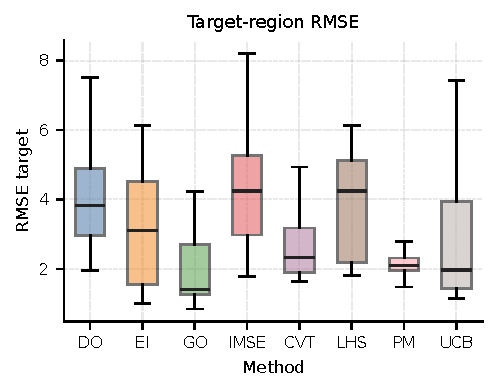
\includegraphics[width=0.45\linewidth]{sub/battery/battery_rmse_target.pdf}}
	\hfill
	\subfigure[\reviewadd{SoC 误差不超过 5\% 的比例。}{R2-5}]{%
		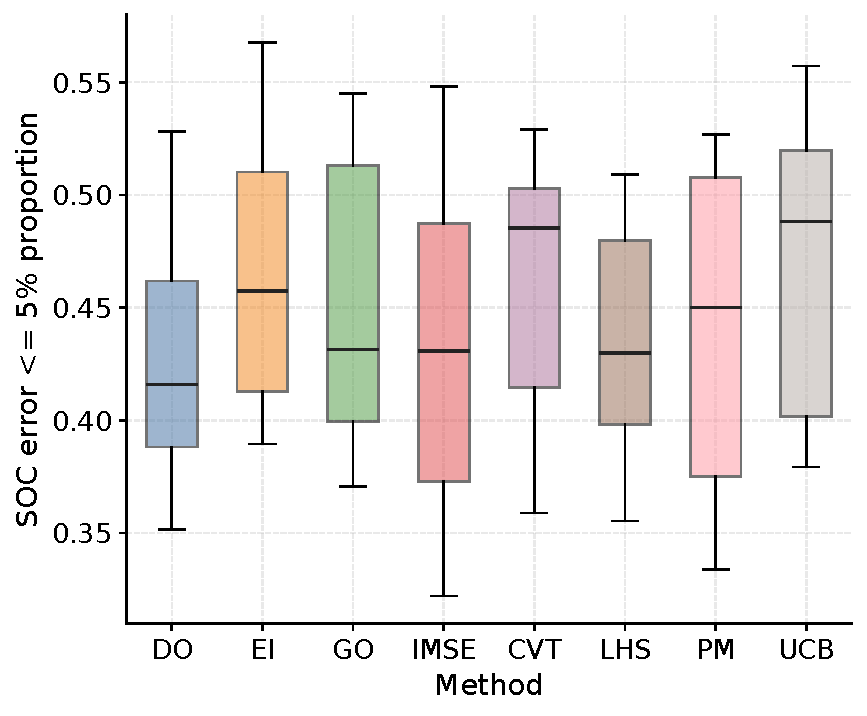
\includegraphics[width=0.45\linewidth]{sub/battery/battery_soc_ratio.pdf}}
	\caption{\reviewadd{电池 SoC 预测结果多指标比较。}{R1-2, R2-4, R2-5}}
	\label{fig:battery_results}
\end{figure}

\reviewadd{表~\ref{tab:battery_results} 表明，PM 方法在目标区域 RMSE 上与 GO 基本持平并略优（均值 2.197 vs. 2.202），明显优于 EI、IMSE 和 UCB 等主动学习基线；同时，PM 的目标区域最大绝对误差均值为 13.903，小于 LHS（21.198）、DO（19.911）、EI（19.523）和 UCB（20.646），说明其对目标 SoC 区间内极端预测误差具有更好的抑制作用。SoC 误差不超过 5\% 的比例方面，各方法差异相对较小，PM 仍保持在 0.442 的合理水平。综合来看，PM 在保持可接受整体误差和工程误差比例的同时，提高了目标区域预测精度并降低了极端误差，更符合稳健参数设计对关键质量区间建模的要求。}{R1-2, R2-4, R2-5}

\reviewadd{\subsection{航空机翼重量工程案例}
为进一步验证所提方法在高维非平稳工程场景中的适用性，本节采用 10 维航空机翼重量（Wing Weight）工程解析基准案例。该案例源自经典航空工程代理建模基准，输入变量包括翼面积（$x_1$，ft$^2$）、燃油重量（$x_2$，lb）、展弦比（$x_3$）、四分之一弦长后掠角（$x_4$，deg）、动压（$x_5$，lb/ft$^2$）、梢根比（$x_6$）、厚度弦长比（$x_7$）、极限载荷因子（$x_8$）、总重（$x_9$，lb）和涂装重量（$x_{10}$，lb）。为引入更具挑战性的非平稳结构，本文在原始 Wing Weight 公式基础上加入高载荷/高动压结构加强项、特定后掠角区间分段修正项以及薄翼高展弦比多峰扰动项，从而形成同时包含高维性、分段突变和多峰局部变化的工程响应面。输出响应为机翼重量（lb）。

该案例中稳健参数设计的目标，是识别一组最优设计参数，使机翼重量达到 $300$ lb 或尽可能接近该目标；目标区域定义为 $|y-300|\le20$ lb，用于评价代理模型在关键质量区间内的预测能力。实验流程与微型火箭案例中的优化评价口径保持一致：首先，各方法均从 $80$ 个初始 LHS 训练点出发，并新增 $30$ 个设计点，最终训练样本数为 $110$；随后，基于各方法得到的训练集拟合 NSGP 代理模型，并采用 genetic algorithm 最小化预测质量损失 $(\hat f(\mathbf{x})-300)^2+v(\mathbf{x})$，其中 $\hat f(\mathbf{x})$ 和 $v(\mathbf{x})$ 分别为预测均值和预测方差。每种方法执行 $20$ 次 GA 优化评价，并用解析 Wing Weight 响应重新计算最优解的真实响应和真实质量损失。比较方法包括 DO、GO、CVT、LHS、PM 以及 EI、IMSE 和 UCB。表~\ref{tab:wing_results} 和图~\ref{fig:wing_results} 汇总了主要优化结果。}{AE-1, R1-5, R2-5, R2-6}

\begin{table}[h!]
	\centering
	\caption{\reviewadd{10 维 Wing Weight 案例优化结果汇总（均值/中位数）。}{AE-1, R1-5, R2-5, R2-6}}
	\label{tab:wing_results}
	\begingroup\color{red}
	\resizebox{\linewidth}{!}{%
		\begin{tabular}{lrrrrrrrr}
			\toprule
			& \multicolumn{2}{c}{RMSE in the target region} & \multicolumn{2}{c}{RMSE over the full surface} & \multicolumn{2}{c}{GA true response} & \multicolumn{2}{c}{True quality loss} \\
			方法 & 均值 & 中位数 & 均值 & 中位数 & 均值 & 中位数 & 均值 & 中位数 \\
			\midrule
			DO   & 10.068 &  9.821 &  9.746 &  9.502 & 294.792 & 294.252 & 49.719 & 34.803 \\
			EI   & 10.670 & 10.695 & 10.299 & 10.358 & 297.681 & 297.980 & 40.413 &  9.967 \\
			GO   &  9.544 &  9.554 &  8.861 &  8.860 & 296.375 & 296.248 & 50.262 & 19.574 \\
			IMSE &  9.403 &  9.390 &  9.969 & 10.052 & 297.325 & 296.291 & 37.378 & 32.810 \\
			CVT  &  9.590 &  9.607 &  9.917 &  9.920 & 295.184 & 294.141 & 65.396 & 42.003 \\
			LHS  &  9.438 &  9.446 &  9.972 &  9.985 & 294.497 & 294.515 & 43.811 & 30.284 \\
			PM   &  8.953 &  8.918 & 10.116 &  9.947 & 299.456 & 299.486 & 17.399 &  6.000 \\
			UCB  & 10.539 & 10.538 & 10.118 & 10.106 & 299.932 & 299.887 & 30.990 & 12.475 \\
			\bottomrule
		\end{tabular}%
	}
	\endgroup
\end{table}

\begin{figure}[h!]
	\centering
	\subfigure[\reviewadd{目标区域 RMSE。}{AE-1, R1-5, R2-6}]{%
		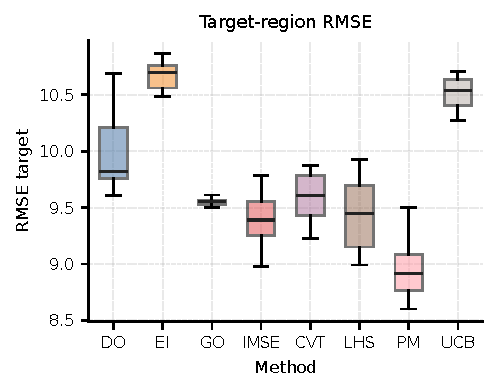
\includegraphics[width=0.48\linewidth]{sub/wing/wing_rmse_target.pdf}}
	\hfill
	\subfigure[\reviewadd{GA 最优解的真实质量损失。}{AE-1, R1-5, R2-5, R2-6}]{%
		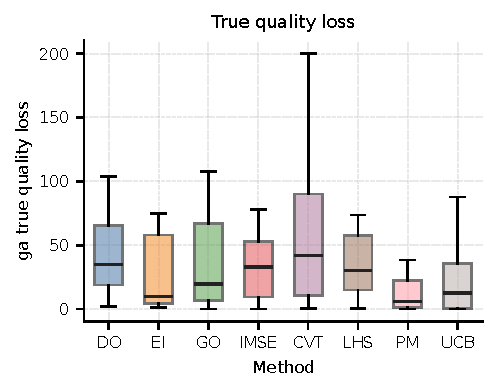
\includegraphics[width=0.48\linewidth]{sub/wing/wing_true_quality_loss.pdf}}
	\caption{\reviewadd{10 维 Wing Weight 案例优化结果：(a) 目标区域 RMSE；(b) GA 最优解的真实质量损失。}{AE-1, R1-5, R2-5, R2-6}}
	\label{fig:wing_results}
\end{figure}

\reviewadd{表~\ref{tab:wing_results} 和图~\ref{fig:wing_results} 表明，PM 方法在目标区域 RMSE 和真实质量损失两项核心指标上均取得最优结果。其目标区域 RMSE 均值为 8.953，低于 LHS（9.438）、GO（9.544）和 UCB（10.539）；真实质量损失均值为 17.399，较 UCB 的 30.990 降低 43.86\%，较 LHS 的 43.811 降低 60.29\%。在 GA 最优解的真实响应方面，PM 的均值和中位数分别为 299.456 lb 和 299.486 lb，均最接近 300 lb 目标值。虽然 PM 在整体响应面 RMSE 上并非最低，但其优化解质量明显更优，说明所提注意力采样能够将有限实验资源集中于稳健优化真正依赖的目标区域，从而提高高维非平稳工程案例中的参数优化可靠性。}{AE-1, R1-5, R2-5, R2-6}

		\subsection{微型火箭稳健参数设计}
	
	本节采用 \cite{Box2011} 提出的微型火箭设计案例，验证所提方法在产品质量设计中的有效性和优势。火箭模型由头锥、箭体、带降落伞的发射阻尼锁、内管和稳定翼组成，如图 7 所示。输出响应为最大飞行高度（MH）$y$（m），是评价火箭整体性能的关键指标。最大高度分析能够综合反映推力、气动阻力和结构设计性能。在该案例中，目标值设为 400 m，代表典型的 nominal-the-best 质量特性。模拟飞行轨迹以及最大飞行高度与头锥直径之间的关系分别见图 8(a) 和 8(b)。

\begin{figure}[h!]
	\centering
	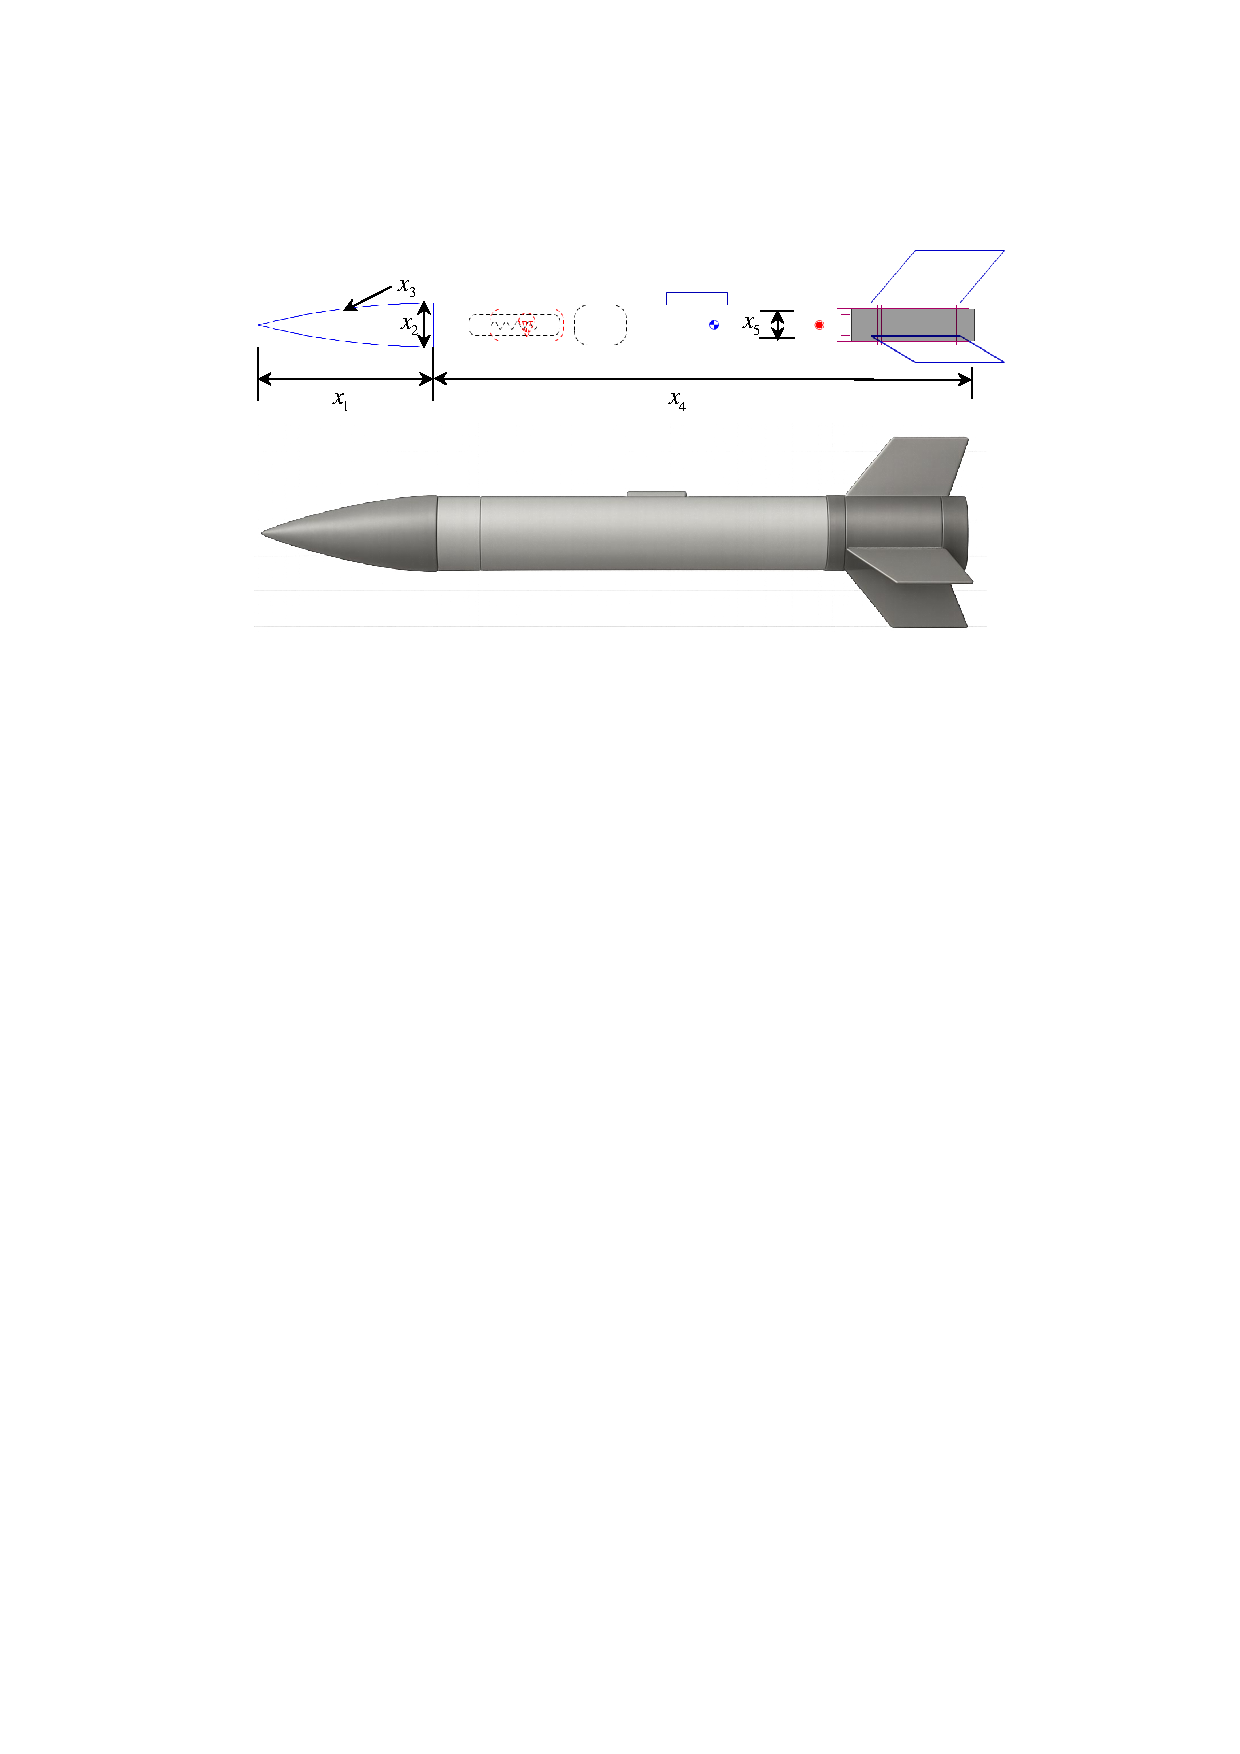
\includegraphics[width=0.7\linewidth]{FIG8.pdf}% 
		\caption{火箭模型示意图。}
		\label{fig:rocket_model}
	\end{figure}
	
	\begin{figure}[h!]
		\centering
		\subfigure[火箭飞行轨迹示意。]{%
			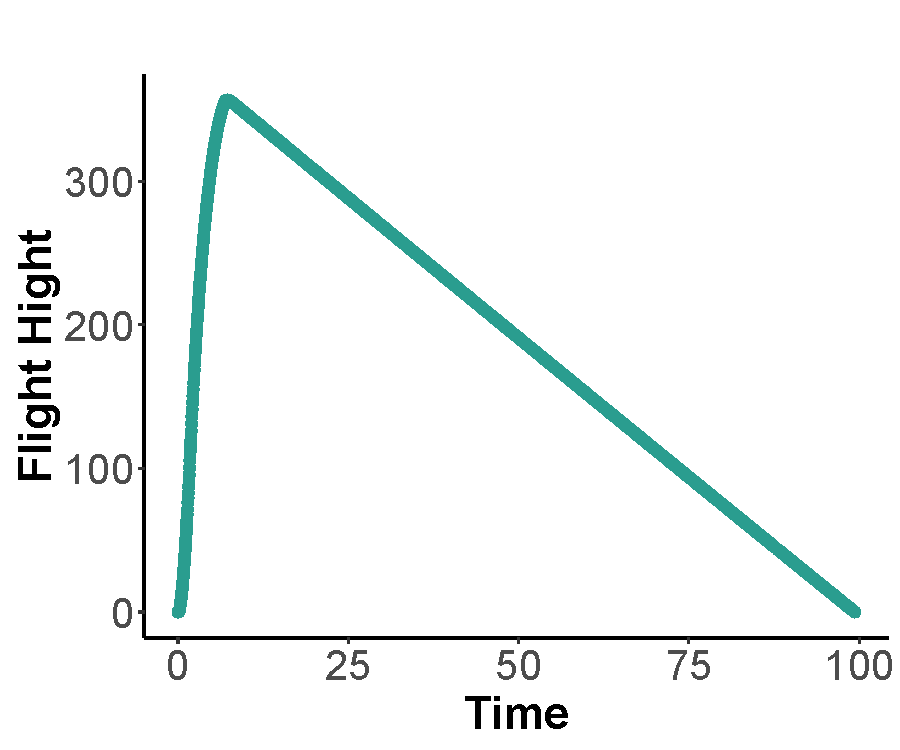
\includegraphics[width=0.48\linewidth]{FIG9a.pdf}%
		}\hspace{5pt}
		\subfigure[MH 与头锥直径。]{%
			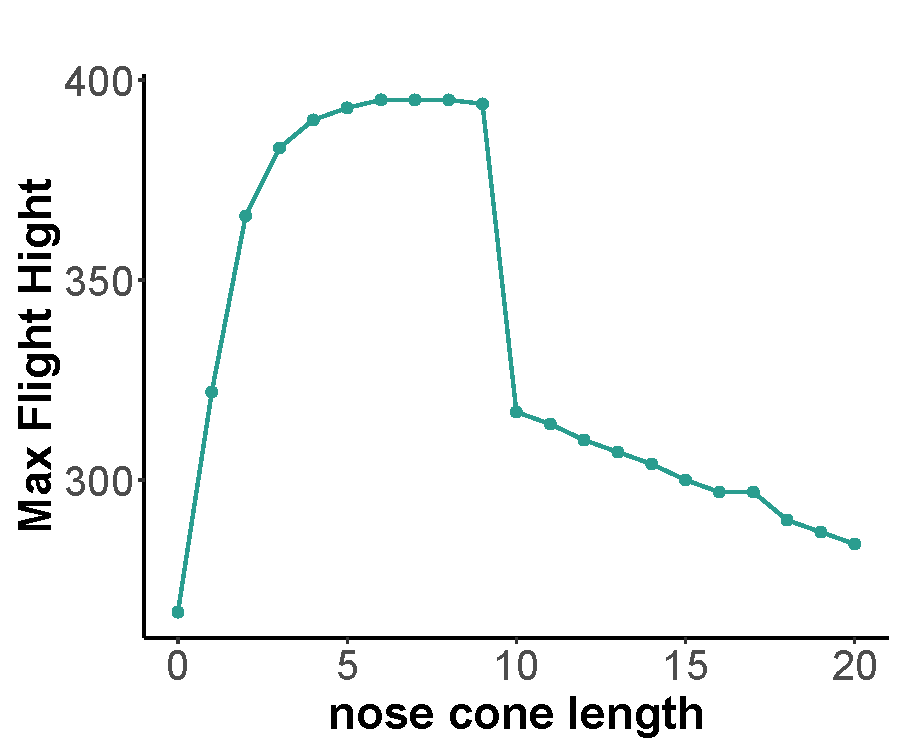
\includegraphics[width=0.48\linewidth]{FIG9b.pdf}%
		}
		\caption{模拟飞行轨迹以及 MH 与头锥直径之间的关系。}
		\label{fig:rocket_traj_pair}
	\end{figure}
	
	该案例包含五个连续输入参数：头锥长度 $x_{1}$（cm）、头锥底部直径 $x_{2}$（cm）、头锥壁厚 $x_{3}$（cm）、箭体长度 $x_{4}$（cm）和箭体内径 $x_{5}$（cm）。其取值范围分别为 $x_{1} \in [0,20]$、$x_{2} \in [2,5]$、$x_{3} \in [0,1]$、$x_{4} \in [30,50]$ 和 $x_{5} \in [1,2]$。此外，还有一个二元离散变量，即头锥形状 $x_{6}$，其中 $x_{6} = 1$ 表示切尖 ogive，$x_{6} = 0$ 表示截尖 ogive。根据设计规范，当头锥较长（$x_{1} > 10$ cm）时，优先采用切尖 ogive，以降低超声速飞行中的激波阻力，从而改善气动性能并提高稳定性；当头锥较短（$x_{1} < 10$ cm）时，采用截尖 ogive，以提高亚声速飞行中的升力和稳定性。$x_{1} = 10$ cm 处的形状转换引入明显结构变化，使输出响应在该位置呈阶跃行为，从而产生显著非平稳特征。
	
	该案例中稳健参数设计的目标，是识别一组最优设计参数，使火箭最大飞行高度达到 $400$ m 或尽可能接近该目标。为此，后续实验采用所提方法提升潜在最优区域内的预测精度，从而构建更高效、更稳定的非平稳响应面模型。实验流程如下：首先，采用 LHS 方法选取 $30$ 个初始训练点，并拟合基于 NSGP 的初始非平稳响应面模型；随后，利用所提两阶段主动学习算法生成 $20$ 个额外设计点，使训练样本总数达到 $50$，如表 5 所示。

\begin{table}[h!]
	\centering
		\caption{PM 方法实验结果。}
		\label{tab:pm_runs}
		\resizebox{\linewidth}{!}{%
			\begin{tabular}{c cccccc c c cccccc cc}
			\toprule
			\multicolumn{8}{c}{运行 1--25} & & \multicolumn{8}{c}{运行 26--50} \\
			\cmidrule(lr){1-8} \cmidrule(lr){10-17}
			运行 & $x_1$ & $x_2$ & $x_3$ & $x_4$ & $x_5$ & $x_6$ & $y$ & & 运行 & $x_1$ & $x_2$ & $x_3$ & $x_4$ & $x_5$ & $x_6$ & $y$ \\
			\midrule
			1 & 15.5 & 3.13 & 0.96 & 48.8 & 1.89 & 1 & 26.7  & & 26 &  9.9 & 2.20 & 0.02 & 38.4 & 1.62 & 0 & 262    \\
			2 & 12.9 & 2.81 & 0.07 & 41.3 & 1.96 & 1 & 130    & & 27 & 14.2 & 2.91 & 0.28 & 38.6 & 1.86 & 1 &  87.5  \\
			3 &  1.3 & 2.06 & 0.63 & 37.4 & 1.31 & 0 & 227    & & 28 & 16.6 & 2.71 & 0.90 & 40.9 & 1.38 & 1 &  50.5  \\
			4 &  0.5 & 3.97 & 0.10 & 45.6 & 1.23 & 0 &  7.59  & & 29 & 17.2 & 3.32 & 0.44 & 30.8 & 1.14 & 1 &  33.6  \\
			5 & 10.7 & 4.17 & 0.13 & 33.9 & 1.86 & 1 &  1.1   & & 30 &  5.2 & 4.50 & 1.00 & 32.0 & 1.54 & 0 &   9.25 \\
			6 & 18.7 & 4.81 & 0.86 & 36.7 & 1.18 & 1 &  0.39  & & 31 &  0.7 & 2.08 & 0.25 & 30.7 & 1.92 & 0 & 373.89 \\
			7 & 17.9 & 3.85 & 0.65 & 47.0 & 1.49 & 1 &  4.59  & & 32 &  4.9 & 2.03 & 0.16 & 34.8 & 1.88 & 0 & 358.91 \\
			8 &  2.6 & 2.39 & 0.83 & 45.5 & 1.53 & 0 & 146    & & 33 &  5.8 & 2.12 & 0.02 & 30.2 & 1.97 & 0 & 369.85 \\
			9 &  2.0 & 4.69 & 0.67 & 32.9 & 1.15 & 0 &  5.65  & & 34 &  8.7 & 2.02 & 0.19 & 33.4 & 1.89 & 0 & 362.51 \\
			10 & 11.1 & 4.97 & 0.14 & 44.2 & 1.92 & 1 &  0.64  & & 35 & 10.5 & 2.03 & 0.35 & 31.3 & 1.86 & 1 & 358.85 \\
			11 & 18.0 & 3.99 & 0.82 & 40.6 & 1.98 & 1 &  7.19  & & 36 &  0.4 & 2.04 & 0.77 & 34.9 & 1.95 & 0 & 365.41 \\
			12 &  2.0 & 2.96 & 0.24 & 42.6 & 1.33 & 0 &  6.25  & & 37 &  4.0 & 2.05 & 0.17 & 32.8 & 1.85 & 0 & 358.41 \\
			13 & 17.3 & 4.63 & 0.91 & 43.3 & 1.00 & 1 &  0.27  & & 38 &  2.1 & 2.08 & 0.45 & 35.6 & 1.99 & 0 & 359.29 \\
			14 & 11.2 & 3.71 & 0.32 & 33.5 & 1.72 & 1 & 29     & & 39 &  6.8 & 2.12 & 0.07 & 33.5 & 1.99 & 0 & 358.02 \\
			15 &  8.1 & 3.75 & 0.50 & 35.8 & 1.69 & 0 & 24.6   & & 40 & 10.3 & 2.03 & 0.08 & 36.1 & 1.89 & 1 & 348.89 \\
			16 & 15.6 & 2.50 & 0.23 & 47.4 & 1.26 & 1 & 77.6   & & 41 &  2.0 & 2.04 & 0.89 & 33.6 & 1.84 & 0 & 349.3  \\
			17 &  7.5 & 3.15 & 0.44 & 31.5 & 1.57 & 0 & 73.3   & & 42 &  3.0 & 2.13 & 0.33 & 31.3 & 1.87 & 0 & 347.57 \\
			18 &  8.8 & 3.45 & 0.70 & 44.6 & 1.81 & 0 & 25.9   & & 43 &  8.1 & 2.04 & 0.85 & 35.0 & 1.90 & 0 & 345.66 \\
			19 & 19.0 & 2.26 & 0.04 & 49.5 & 1.47 & 1 & 159    & & 44 &  4.3 & 2.12 & 1.00 & 30.4 & 1.90 & 0 & 350.13 \\
			20 &  6.8 & 4.13 & 0.50 & 36.1 & 1.44 & 0 & 11.8   & & 45 &  7.8 & 2.00 & 0.93 & 30.4 & 1.82 & 0 & 360.47 \\
			21 & 11.9 & 3.55 & 0.84 & 42.0 & 1.74 & 1 & 17.3   & & 46 &  8.4 & 2.02 & 0.55 & 32.3 & 1.89 & 0 & 365.2  \\
			22 &  6.6 & 3.58 & 0.80 & 37.9 & 1.06 & 0 & 19.4   & & 47 & 11.8 & 2.09 & 0.14 & 32.0 & 1.86 & 1 & 340.6  \\
			23 &  2.9 & 2.01 & 0.76 & 47.8 & 1.74 & 0 & 306    & & 48 & 19.8 & 2.01 & 0.82 & 34.2 & 1.97 & 1 & 353.39 \\
			24 & 13.4 & 2.35 & 0.10 & 39.8 & 1.22 & 1 & 139    & & 49 & 12.9 & 2.04 & 0.72 & 35.0 & 1.90 & 1 & 342.23 \\
			25 &  8.7 & 2.18 & 0.54 & 40.2 & 1.03 & 0 & 147    & & 50 & 14.0 & 2.00 & 0.40 & 36.3 & 1.88 & 1 & 341.54 \\
			\bottomrule
			\end{tabular}}
	\end{table}
	
	如表 5 所示，所提方法能够使新增加的第 31--50 个实验点响应值接近 400 的目标值。同时，这些点在设计空间中分布均匀，没有明显聚集或重叠。该结果验证了所提两阶段主动学习建模方法在兼顾空间填充和目标聚焦采样方面的有效性。基于表 5 中的实验数据，构建 NSGP 模型，并利用其输出建立稳健优化模型：
	\begin{equation}
		L({\bf{x}}) = {\left( {f({\bf{x}}) - 400} \right)^2} + v({\bf{x}}),
	\end{equation}
	其中，$f(\mathbf{x})$ 为预测响应，$v(\mathbf{x})$ 为预测方差，$400$ 为预设最优目标值。随后采用 genetic algorithm 最小化式（33），得到最优输入参数配置。算法参数设定如下：初始种群规模为 $50$，最大迭代次数为 $200$，停止阈值为 $20$，其余参数保持默认。优化过程重复 $30$ 次，并记录每种方法的实际 MH、质量损失（QL）值以及模拟火箭飞行轨迹。结果见表 6 和图 9。此外，为评估不同初始样本量的影响，附录 B 给出了初始训练样本为 $40$、$50$ 和 $60$ 时的比较结果（对应总训练样本分别为 $60$、$70$ 和 $80$）。

\begin{table}[h!]
	\centering
		\caption{不同方法的 MH 和 QL。}
		\label{tab:mh_ql}
		\resizebox{\linewidth}{!}{%
			\begin{tabular}{lcccccccccccc}
			\toprule
			\multirow{2}{*}{方法} & \multicolumn{2}{c}{均值} & \multicolumn{2}{c}{中位数} & \multicolumn{2}{c}{最大值} & \multicolumn{2}{c}{最小值} & \multicolumn{2}{c}{Q1} & \multicolumn{2}{c}{Q3} \\
			\cmidrule(lr){2-3} \cmidrule(lr){4-5} \cmidrule(lr){6-7} \cmidrule(lr){8-9} \cmidrule(lr){10-11} \cmidrule(lr){12-13}
			& MH & QL & MH & QL & MH & QL & MH & QL & MH & QL & MH & QL \\
			\midrule
			PM     & 365.60 & 1908.09 & 373.00 & 1456.03 & 391.00 & 4798.06 & 303.00 &   91.75 & 348.25 & 1128.42 & 381.75 & 2967.72 \\
			LHS    & 351.60 & 4496.26 & 356.00 & 4166.58 & 379.00 & 13731.95 & 287.00 & 1279.43 & 347.25 & 2767.04 & 364.25 & 5655.17 \\
			CVT    & 327.33 & 8549.50 & 332.50 & 8538.47 & 381.00 & 15838.97 & 248.00 & 1719.21 & 308.75 & 5774.53 & 349.50 & 11256.48 \\
				DO & 338.27 & 6099.77 & 344.50 & 5423.04 & 373.00 & 20689.30 & 217.00 & 1076.50 & 326.50 & 4158.41 & 359.25 & 6954.43 \\
				GO & 345.90 & 5288.10 & 347.50 & 4660.24 & 379.00 & 16077.51 & 275.00 &  271.08 & 330.25 & 3033.79 & 370.75 & 7422.89 \\
				\bottomrule
			\end{tabular}%
		}
	\end{table}
	
	\begin{figure}[h!]
		\centering
		% --- First row: MH and QL ---
		\subfigure[MH。]{%
			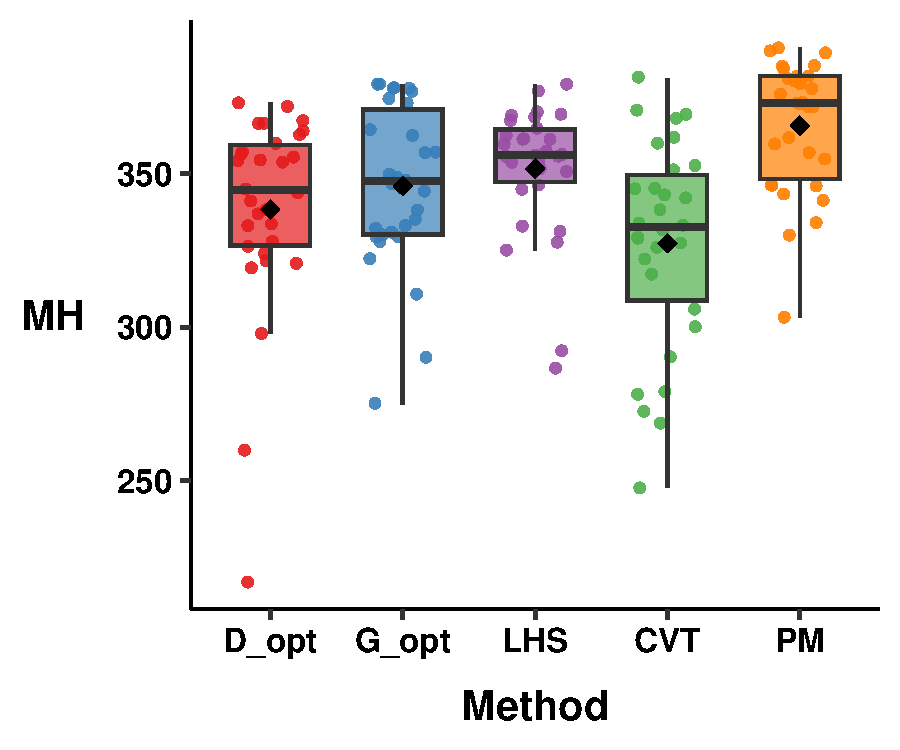
\includegraphics[width=0.48\linewidth]{FIG10a.pdf}}
		\hfill
		\subfigure[QL。]{%
			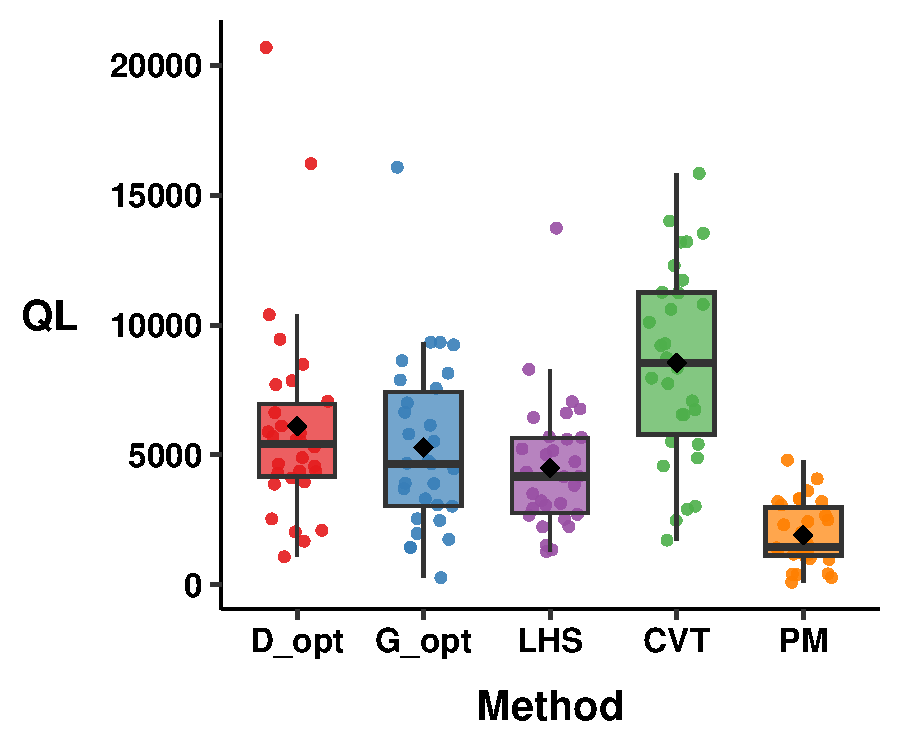
\includegraphics[width=0.48\linewidth]{FIG10b.pdf}}
		
		% --- Second row: Flight trajectories ---
		\vskip\baselineskip
		\subfigure[飞行轨迹。]{%
			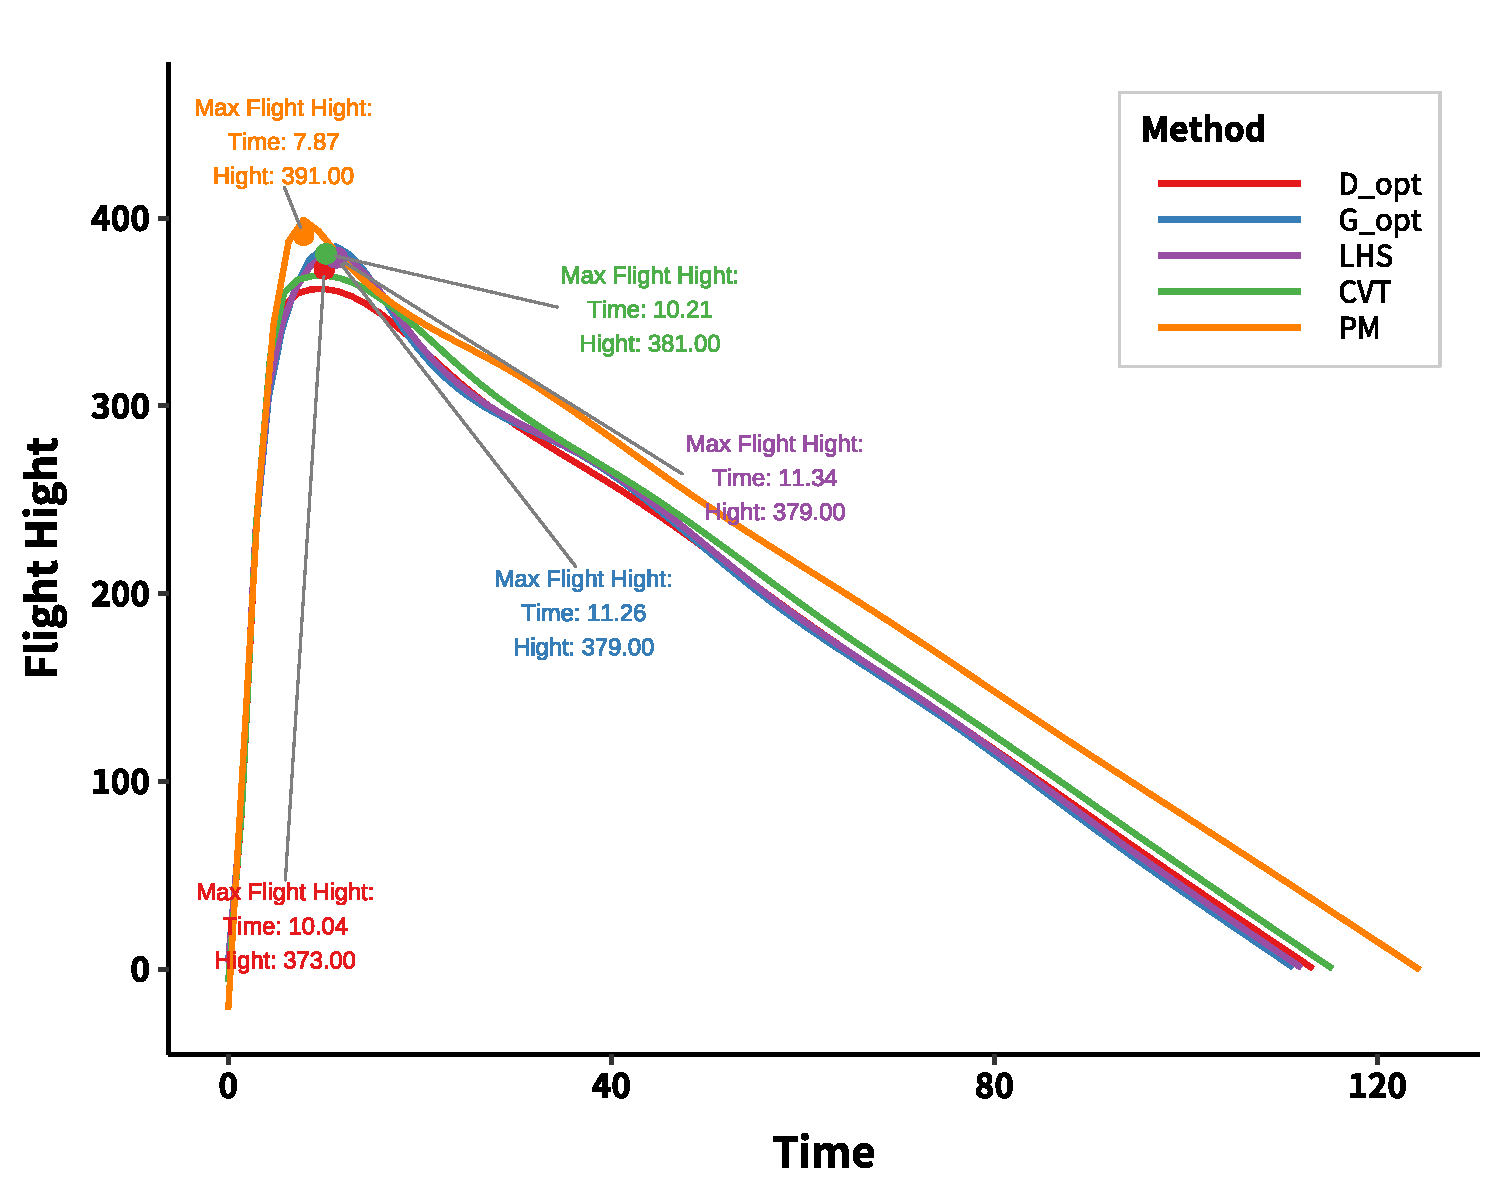
\includegraphics[width=\linewidth]{FIG11.pdf}}
		
		\caption{不同方法的优化结果：
			(a) MH；(b) QL；(c) 飞行轨迹。}
		\label{fig:optimization_results}
	\end{figure}
	
	图 9(a-b) 清晰展示了不同方法在 MH 和 QL 指标上的性能差异。相较于其他方法，所提 PM 方法取得了更高的 MH 均值和中位数，且离群点更少，说明优化过程具有更强稳健性。对于 QL，PM 方法的均值和中位数均低于其他方法，30 次实验结果也更集中、波动更小，体现了更优的优化性能和稳定性。
	
	如表 6 所示，PM 方法在所有指标上均表现优越。相较 LHS 方法，其 QL 均值从 4496.26 降至 1908.09（降低 57.56\%），中位数降低 65.05\%；最大和最小 QL 分别降低 65.06\% 和 92.83\%。对于 MH，均值（365.6）和中位数（373）分别提高 3.98\% 和 4.78\%，最大值和最小值分别提高 3.17\% 和 5.57\%。相较 CVT 方法，PM 方法的 QL 均值和中位数分别降低 22.30\% 和 82.95\%，MH 均值和最小值分别提高 11.69\% 和 22.18\%。相较 D\-opt 方法，QL 最大值和均值分别降低 76.81\% 和 68.72\%，MH 均值和中位数分别提高 8.08\% 和 8.27\%。相较 G\-opt 方法，QL 均值、中位数和最小值分别降低 63.92\%、68.76\% 和 66.16\%，MH 均值和中位数分别提高 5.69\% 和 7.34\%，最大值和最小值分别提高 3.17\% 和 10.18\%。
	
	结果表明，带注意力机制的两阶段主动学习算法能够更准确捕捉潜在最优区域内的响应面，并提高设计点利用效率。这一改进显著增强了响应面模型在稳健参数设计中的有效性，并提高了最优解的稳健性和可靠性。
	
	本文将 30 次优化运行中取得最高最大飞行高度的设计确定为最优解。图 9(c) 展示了不同方法所得最优解的 MH 值及其对应飞行轨迹。相较其他方法，PM 方法在 MH 方面表现最佳，达到 391 m，更接近 400 m 目标值。就飞行时间而言，各方法均在约 7.5 s 达到峰值高度，并在约 122 s 返回地面。然而，其他方法的 MH 值明显低于 PM 方法。轨迹剖面对比表明，尽管各方法上升持续时间几乎相同，PM 方法仍提供了更接近目标值的稳健最优解，从而提高产品质量改进效率。

\subsection{讨论}
本文提出一种基于注意力机制的两阶段主动学习算法。其核心在于构建一个能够动态关注潜在最优区域和设计点空间填充性能的注意力模型。该机制引导新增设计点以优先且均衡的方式分配至目标子区域。因此，潜在最优区域内的预测精度得到显著提升，进而增强最优解的稳健性和有效性。

\reviewadd{消融实验确认了所提两阶段结构的必要性：单独使用质量损失或空间填充均会导致性能退化，softmax 归一化对平滑权重分布和抑制极端选择具有重要作用。目标值敏感性分析表明，只要采样目标 $T$ 与真实目标不存在数量级偏差，PM 方法的性能保持稳定。通过与 EI、UCB、IMSE 等现代主动学习采集函数的广泛对比，PM 方法在目标区域精度和优化质量上均展现出显著优势。10 维 Wing Weight 案例进一步验证了方法在高维非平稳工程场景中的可扩展性和有效性。}{R1-1, R2-1, R2-2, R2-3, R1-2, R2-4, R2-6}

虽然该方法以全局预测精度小幅下降为代价强化局部建模，但这并不削弱其整体有效性。\reviewadd{如表 2 和表 4 所示，PM 方法在目标区域 RMSE（RMSE in the target region）上的下降幅度（例如 10 个主动学习点、$n=100$ 时相较 DO 降低 19.56\%）远大于其在整体 RMSE（RMSE over the full surface）上的增加幅度（仅增加约 0.0116），验证了局部精度提升的净收益。}{R1-3}由于潜在最优区域内的精度在很大程度上决定优化质量，将计算和实验资源集中于该区域对于有效稳健优化至关重要。

\reviewadd{关于计算成本，PM 方法的主要开销来自 NSGP 模型反复拟合（每次拟合需运行 HMC 采样）、候选点采集函数计算和 maximin 距离计算。在二维算例的 30 次重复实验中，完整 PM（含 20 个主动学习点、总样本 70）的平均运行时间约 158 秒，与 EI（约 157 秒）、UCB（约 157 秒）和 IMSE（约 158 秒）基本持平。模型拟合时间占总时间的 95\% 以上，采集函数本身计算开销可忽略。这一结果说明 PM 方法在以 HMC 为基础的非平稳 GP 建模中未引入显著的额外计算负担。}{R1-4}

\section{结论}
针对小样本条件下非平稳响应的质量改进问题，本文提出一种基于注意力主动学习的 NSGP 建模与稳健优化框架。首先，采用 Bayesian 层次化设定构建 NSGP 结构，刻画设计变量与输出响应之间的输入依赖非平稳性。其次，设计两阶段注意力机制以平衡质量损失与空间填充，引导新设计点向潜在最优区域聚集。最后，更新训练集和 NSGP 模型，并构造基于质量损失的稳健优化模型，以获得最优输入参数设置。\reviewadd{通过二维基准测试、锂电池 SoC 预测、Wing Weight 10 维工程案例和微型火箭稳健参数设计四个案例的系统验证，以及消融实验和敏感性分析的支撑，}{AE-1}\reviewadd{与 EI、UCB、IMSE 等现代主动学习方法的对比进一步证明了 PM 的竞争力。}{R1-2, R2-4}该方法的关键优势在于两阶段注意力加权采样策略，它能够高效识别非平稳响应的潜在最优区域，将实验资源分配至该区域，并提升优化关键区域的预测精度。

需要指出的是，所提方法采用聚焦式注意力策略，优先提升潜在最优区域的预测精度，以提高稳健参数设计效率。全局预测精度并非显式目标，这可能限制其在其他优化任务中的适用性。未来研究可探索同时考虑全局与局部精度的多层次注意力机制，以进一步扩展所提方法的适用范围。\reviewadd{此外，可研究将深度核学习或 transformer 架构引入非平稳 GP 建模，以进一步提升模型表达能力。}{R1-6, R2-7}


\section*{利益冲突声明}

作者声明不存在竞争性利益。


\section*{基金资助}

本文得到国家自然科学基金（项目编号 72301146）、中国博士后科学基金（项目编号 2023M741802、2024T170430）、中国统计科学研究基金（项目编号 2023LZ010）以及江苏省高等学校自然科学研究项目（项目编号 23KJB630012）资助。


\section*{作者简介}
\begin{itemize}
 \item 冯泽彪于 2021 年在南京理工大学经济管理学院获得博士学位，现为南京邮电大学管理学院助理教授。研究方向包括质量工程、计算机实验和机器学习。

 \item 杨旭目前在南京邮电大学管理学院攻读管理科学与工程硕士学位。研究方向包括质量工程和机器学习。
 
 \item 王建军现为南京理工大学经济管理学院教授，博士毕业于南京理工大学经济管理学院。研究方向包括质量工程、应用统计和增材制造。

 \item 黄卫东现任南京邮电大学管理学院院长、教授，博士毕业于南京航空航天大学计算机科学与技术专业。主要研究方向包括智能优化、决策和应急管理。
\end{itemize}

\section*{数据可用性声明}

作者确认，支撑本文研究结论的数据均可在正文中获得。


\begin{thebibliography}{}

\bibitem[Alshraideh and del Castillo(2014)]{Alshraideh2014}
Alshraideh, H., and E. del Castillo. 2014. ``Gaussian process modeling and optimization of profile response experiments.'' \emph{Quality and Reliability Engineering International} 30 (4): 449--462.

\bibitem[An et~al.(2020)]{An2020}
An, Y., D. Wang, and X. Zhang. 2020. ``A novel local temperature change detection approach in a 3D thermal field.'' \emph{Quality Technology \& Quantitative Management} 17 (6): 723--737.

\bibitem[Ankenman et~al.(2010)]{Ankenman2010}
Ankenman, B., B. L. Nelson, and J. Staum. 2010. ``Stochastic Kriging for simulation metamodeling.'' \emph{Operations Research} 58 (2): 371--382.

\bibitem[Bao et~al.(2016)]{Bao2016}
Bao, L. L., Q. Huang, and K. B. Wang. 2016. ``Robust parameter design for profile quality control.'' \emph{Quality and Reliability Engineering International} 32 (3): 1059--1070.

\bibitem[Barde(2024)]{Barde2024}
Barde, S.. 2024. ``Bayesian estimation of large-scale simulation models with Gaussian process regression surrogates.'' \emph{Computational Statistics \& Data Analysis} 196: 107972.

\bibitem[Box, et~al.(2011)]{Box2011}
Box, S., C. M. Bishop, and H. Hunt. 2011. ``Stochastic six-degree-of-freedom flight simulator for passively controlled high-power rockets.'' \emph{Journal of Aerospace Engineering} 24 (1): 31--45.

\bibitem[Chen and Tuo(2022)]{Chen2022}
Chen, G., and R. Tuo. 2022. ``Projection pursuit Gaussian process regression.'' \emph{IISE Transactions} 55 (9): 901--911.

\bibitem[Chen et~al.(2021)]{Chen2021}
Chen, J. H., L. L. Kang, and G. Lin. 2021. ``Gaussian process assisted active learning of physical laws.'' \emph{Technometrics} 63 (3): 329--342.

\bibitem[Chuang and Wu(2017)]{Chuang2017}
Chuang, C. J., and C. W. Wu. 2017. ``Determining optimal process mean and quality improvement in a profit-maximization supply chain model.'' \emph{Quality Technology \& Quantitative Management} 16 (2): 154--169.

\bibitem[Davis et~al.(2021)]{Davis2021}
Davis, C. B., C. M. Hans, and T. J. Santner. 2021. ``Prediction of non-stationary response functions using a Bayesian composite Gaussian process.'' \emph{Computational Statistics \& Data Analysis} 154: 107083.

\bibitem[Dellino et~al.(2012)]{Dellino2012}
Dellino, G., J. P. C. Kleijnen, and C. Meloni. 2012. ``Robust optimization in simulation: Taguchi and Krige combined.'' \emph{INFORMS Journal on Computing} 24 (3): 471--484.

\bibitem[Ding et~al.(2024)]{Ding2024}
Ding, N., Z. He, S. He, and L. Song. 2024. ``Real-time profile monitoring schemes considering covariates using Gaussian process via sensor data.'' \emph{Quality Technology \& Quantitative Management} 21 (1): 35--53.

\bibitem[Ding et~al.(2004)]{Ding2004}
Ding, R., D. K. J. Lin, and D. Wei. 2004. ``Dual-response surface optimization: a weighted MSE approach.'' \emph{Quality Engineering} 16 (3): 377--385.

\bibitem[Fan(2000)]{Fan2000}
Fan, S. K. S. 2000. ``A generalized global optimization algorithm for dual response systems.'' \emph{Journal of Quality Technology} 32 (4): 444--456.

\bibitem[Feng et~al.(2021)]{Feng2021}
Feng, Z., J. Wang, Y. Ma, and Y. Tu. 2021. ``Robust parameter design based on Gaussian process with model uncertainty.'' \emph{International Journal of Production Research} 59 (9): 2772--2788.

\bibitem[Feng et~al.(2025)]{Feng2025}
Feng, Z., J. Wang and W. Huang. 2025. ``An active learning multi-objective robust optimization framework via Gaussian process models under uncertainty.'' \emph{Engineering Optimization}: 1-24.

\bibitem[Gelman et~al.(2013)]{Gelman2013}
Gelman, A., H. S. Stern, J. B. Carlin, D. B. Dunson, A. Vehtari, and D. B. Rubin. 2013. \emph{Bayesian Data Analysis}. Chapman and Hall/CRC.

\bibitem[Gnanasambandam et~al.(2024)]{Gnanasambandam2024}
Gnanasambandam, R., B. Shen, A. C. C. Law, C. Dou, and Z. Kong. 2024. ``Deep Gaussian process for enhanced Bayesian optimization and its application in additive manufacturing.'' \emph{IISE Transactions}: 1--14.

\bibitem[Gramacy and Lee(2008)]{Gramacy2008}
Gramacy, R. B., and H. K. H. Lee. 2008. ``Bayesian treed Gaussian process models with an application to computer modeling.'' \emph{Journal of the American Statistical Association} 103 (483): 1119--1130.

\bibitem[Guo et~al.(2023)]{Guo2023}
Guo, B., X. Li, M. Liu, and X. Yang. 2023. ``Construction of orthogonal general sliced Latin hypercube designs.'' \emph{Statistical Papers} 64 (3): 987--1014.

\bibitem[Han et~al.(2023)]{Han2021}
Han, M., Q. Huang, L. Ouyang, and X. Zhao. 2023. ``A kriging-based active learning algorithm for contour estimation of integrated response with noise factors.'' \emph{Engineering with Computers} 39(2): 1341--1362.

\bibitem[Han and Tan(2016)]{Han2016}
Han, M., and M. H. Y. Tan. 2016. ``Integrated parameter and tolerance design with computer experiments.'' \emph{IIE Transactions} 48 (11): 1004--1015.

\bibitem[He et~al.(2021)]{He2021}
He, Z., Y. Gao, L. Qu, and Z. Wang. 2021. ``A nonparametric CUSUM scheme for monitoring multivariate time-between-events-and-amplitude data with application to automobile painting.'' \emph{International Journal of Production Research} 60 (18): 5432--5449.

\bibitem[Heinonen et~al.(2016)]{Heinonen2016}
Heinonen, M., H. Mannerström, J. Rousu, S. Kaski, and H. Lähdesmäki. 2016. ``Non-stationary Gaussian process regression with Hamiltonian Monte Carlo.'' \emph{PMLR}: 732--740.

\bibitem[Hoffman and Gelman(2014)]{Hoffman2014}
Hoffman, M. D., and A. Gelman. 2014. ``The No-U-Turn sampler: adaptively setting path lengths in Hamiltonian Monte Carlo.'' \emph{Journal of Machine Learning Research} 15 (1): 1593--1623.

\bibitem[Huang(2022)]{Huang2022}
Huang, Q.. 2022. ``An impulse response formulation for small-sample learning and control of additive manufacturing quality.'' \emph{IISE Transactions} 55 (9): 926--939.

\bibitem[Jiang and Tan(2021)]{Jiang2021}
Jiang, F., and M. H.-Y. Tan. 2021. ``Shifted log loss Gaussian process model for expected quality loss prediction in robust parameter design.'' \emph{Quality Technology \& Quantitative Management} 18 (5): 527--551.

\reviewadd{
\bibitem[Jones et~al.(1998)]{Jones1998}
Jones, D. R., M. Schonlau, and W. J. Welch. 1998. ``Efficient global optimization of expensive black-box functions.'' \emph{Journal of Global Optimization} 13 (4): 455--492.
}{R1-2, R2-7}

\bibitem[Kleijnen and Mehdad(2014)]{Kleijnen2014}
Kleijnen, J. P. C., and E. Mehdad. 2014. ``Multivariate versus univariate Kriging metamodels for multi-response simulation models.'' \emph{European Journal of Operational Research} 236 (2): 573--582.

\bibitem[Konomi et~al.(2014)]{Konomi2014}
Konomi, B., G. Karagiannis, A. Sarkar, X. Sun, and G. Lin. 2014. ``Bayesian treed multivariate Gaussian process with adaptive design: Application to a carbon capture unit.'' \emph{Technometrics} 56 (2): 145--158.

\bibitem[Li et~al.(2025a)]{Li2025}
Li, A., Z. He, Q. Wang, Y. Zhang, and Y. Ma. 2025a. ``A multi-objective evolutionary algorithm with mutual-information-guided improvement phase for feature selection in complex manufacturing processes.'' \emph{European Journal of Operational Research} 323 (3): 952--965.

\bibitem[Li and Ma(2022)]{Li2022}
Li, T., and J. Ma. 2022. ``Attention mechanism based mixture of Gaussian processes.'' \emph{Pattern Recognition Letters} 161: 130--136.

\bibitem[Li et~al.(2025b)]{Liw2025}
Li, W., J. Qin, C. Wu and F. Tsung. 2025b. ``Online monitoring of directed count-weighted network with attributes via the gravity model.''  \emph{Quality Technology \& Quantitative Management}: 1-16.

\bibitem[Li and Zhou(2016)]{Li2016}
Li, Y., and Q. Zhou. 2016. ``Pairwise meta-modeling of multivariate output computer models using nonseparable covariance function.'' \emph{Technometrics} 58 (4): 483--494.

\bibitem[Lichota(2016)]{Lichota2016}
Lichota, P.. 2016. ``Inclusion of the DOimality in multisine manoeuvre design for aircraft parameter estimation.'' \emph{Journal of Theoretical and Applied Mechanics} 54 (1): 87--98.

\bibitem[Liu et~al.(2021)]{Liu2021}
Liu, Y., D. Huang, B. Liu, Q. Feng, and B. Cai. 2021. ``Adaptive ranking based ensemble learning of Gaussian process regression models for quality-related variable prediction in process industries.'' \emph{Applied Soft Computing} 101: 107060.

\bibitem[Liu et~al.(2025)]{Liu2025}
Liu, Z., Y. Li, X. Yue, and E. Pan. 2025. ``Latent functional Gaussian process incorporating output spatial correlations.'' \emph{IISE Transactions}: 1--14.

\bibitem[Meng et~al.(2022)]{Meng2022}
Meng, Q., S. Wang, and S. H. Ng. 2022. ``Combined global and local search for optimization with Gaussian process models.'' \emph{INFORMS Journal on Computing} 34 (1): 622--637.

\bibitem[Mustafa et~al.(2024)]{Mustafa2024}
Mustafa, H., C. Bourelly, M. Vitelli, F. Milano, M. Molinara, and L. Ferrigno. 2024. ``SoC estimation on Li-ion batteries: A new EIS-based dataset for data-driven applications.'' \emph{Data Brief} 57: 110947.

\bibitem[Omwando(2024)]{Omwando2024}
Omwando, C. N.. 2024. ``G-criterion for second order rotatable designs constructed using trigonometric transformations.'' \emph{American Journal of Applied Mathematics and Statistics} 12 (3): 70--74.

\bibitem[Ouyang et~al.(2025)]{Ouyang2025}
Ouyang, L., Y. Ling, L. Liu, M. Sun, and M. Wang. 2025. ``Double-robust Bayesian variable selection and model prediction with spherically symmetric error.'' \emph{IISE Transactions}: 1--26.

\bibitem[Ouyang et~al.(2016)]{Ouyang2016}
Ouyang, L., Y. Ma, J. H. Byun, J. Wang, and Y. Tu. 2016. ``An interval approach to robust design with parameter uncertainty.'' \emph{International Journal of Production Research} 54 (11): 3201--3215.

\bibitem[Peterson et~al.(2009)]{Peterson2009}
Peterson, J. J., G. Mir{\'o}-Quesada, and E. del Castillo. 2009. ``A Bayesian reliability approach to multiple response optimization with seemingly unrelated regression models.'' \emph{Quality Technology \& Quantitative Management} 6 (4): 353--369.

\bibitem[Rhode(2020)]{Rhode2020}
Rhode, S.. 2020. ``Non-stationary Gaussian process regression applied in validation of vehicle dynamics models.'' \emph{Engineering Applications of Artificial Intelligence} 93: 103716.

\reviewadd{
\bibitem[Sacks et~al.(1989)]{Sacks1989}
Sacks, J., W. J. Welch, T. J. Mitchell, and H. P. Wynn. 1989. ``Design and analysis of computer experiments.'' \emph{Statistical Science} 4 (4): 409--435.
}{R1-2, R2-7}

\bibitem[Santner et~al.(2018)]{Santner2018}
Santner, T. J., B. J. Williams, and W. I. Notz. 2018. \emph{Space-filling designs for computer experiments}. New York: Springer.

\bibitem[Sauer et~al.(2022)]{Sauer2022}
Sauer, A., R. B. Gramacy, and D. Higdon. 2022. ``Active learning for deep Gaussian process surrogates.'' \emph{Technometrics} 65 (1): 4--18.

\reviewadd{
\bibitem[Srinivas et~al.(2010)]{Srinivas2010}
Srinivas, N., A. Krause, S. M. Kakade, and M. Seeger. 2010. ``Gaussian process optimization in the bandit setting: No regret and experimental design.'' In \emph{Proceedings of the 27th International Conference on Machine Learning}: 1015--1022.
}{R1-2, R2-7}

\bibitem[Tan and Wu(2012)]{Tan2012}
Tan, M. H. Y., and C. F. J. Wu. 2012. ``Robust design optimization with quadratic loss derived from Gaussian process models.'' \emph{Technometrics} 54 (1): 51--63.

\bibitem[Vassiliades et~al.(2018)]{Vassiliades2018}
Vassiliades, V., K. Chatzilygeroudis, and J. Mouret. 2018. ``Using centroidal voronoi tessellations to scale up the multidimensional archive of phenotypic elites algorithm.'' \emph{IEEE Transactions on Evolutionary Computation} 22 (4): 623--630.

\bibitem[Wang et~al.(2025)]{Wang2025}
Wang, C., J. Xiao, X. Huang, and J. Xu. 2025. ``RSDS: an efficient adaptive Kriging-based method for structural reliability analysis considering the distance between sample points.'' \emph{Quality Technology \& Quantitative Management}: 1--27.

\bibitem[Wang et~al.(2019)]{Wang2019}
Wang, H., J. Yuan, and S. H. Ng. 2019. ``Gaussian process based optimization algorithms with input uncertainty.'' \emph{IISE Transactions} 52 (4): 377--393.

\bibitem[Wang et~al.(2022)]{Wang2022}
Wang, W., X. Yue, B. Haaland, and C. F. J. Wu. 2022. ``Gaussian processes with input location error and applications to the composite parts assembly process.'' \emph{SIAM/ASA Journal on Uncertainty Quantification} 10 (2): 619--650.

\bibitem[Williams and Rasmussen(2006)]{Williams2006}
Williams, C. K. I., and C. E. Rasmussen. 2006. \emph{Gaussian Processes for Machine Learning}. Cambridge: MIT Press.

\bibitem[Wu and Hamada(2011)]{Wu2011}
Wu, C. F. J., and M. S. Hamada. 2011. \emph{Experiments: Planning, Analysis and Parameter Design Optimization}. New York: John Wiley \& Sons.

\bibitem[Wu et~al.(2020)]{Wu2020}
Wu, C. W., M. H. Shu, and N. Y. Wu. 2020. ``Acceptance sampling schemes for two-parameter Lindley lifetime products under a truncated life test.'' \emph{Quality Technology \& Quantitative Management} 18 (3): 382--395.

\bibitem[Xie et~al.(2022)]{Xie2022}
Xie, J., Z. Ma, D. Chang, G. Zhang, and J. Guo. 2022. ``GPCA: A probabilistic framework for Gaussian process embedded channel attention.'' \emph{IEEE Transactions on Pattern Analysis and Machine Intelligence} 44 (11): 8230--8248.

\bibitem[Yu et~al.(2022)]{Yu2022}
Yu, J., S. Li, X. Liu, Y. Gao, S. Wang, and C. Liu. 2022. ``Dynamic convolutional gated recurrent unit attention auto-encoder for feature learning and fault detection in dynamic industrial processes.'' \emph{International Journal of Production Research} 61 (21): 7434--7452.

\bibitem[Zhang et~al.(2024)]{Zhang2024}
Zhang, W., Z. Zhao, H. Xu, X. Li, and Z. Wang. 2024. ``AK-Gibbs: An active learning Kriging model based on Gibbs importance sampling algorithm for small failure probabilities.'' \emph{Computer Methods in Applied Mechanics and Engineering} 426: 116992.

\bibitem[Zhong et~al.(2024)]{Zhong2024}
Zhong, Y., Z. Ling, L. Liu, S. Zhang, and H. Wen. 2024. ``Deep Gaussian attention network for lumber surface defect segmentation.'' \emph{IEEE Transactions on Instrumentation and Measurement} 73: 1--12.

\bibitem[Zhou et~al.(2025)]{Zhou2025}
Zhou, M., R. Zuo, C. Sung, Y. Tong, and X. Wang. 2025. ``Region-optimal Gaussian process surrogate model via Dirichlet process for cold-flow and combustion emulations.'' \emph{Computer Methods in Applied Mechanics and Engineering} 439: 117894.

\end{thebibliography}


\section{附录}

\appendix

\reviewadd{附录 A 包含二维算例各方法在潜在最优区域内的完整 RMSE 统计量（含 8 种方法的中位数、最小值、最大值、Q1、Q3），按训练样本总数（40--100）列出。附录 B 包含火箭案例不同初始样本量下的优化结果比较。}{R1-2, R2-4}

\section{ }

\begin{table}[h!]
	\centering
	\caption{\reviewadd{10 个主动学习样本，40 个总样本下目标区域 RMSE 完整统计量。}{R1-2, R2-4}}
	\label{tab:app_a1}
	\begin{tabular}{l rrrrr}
		\toprule
		方法 & 中位数 & 最小值 & 最大值 & Q1 & Q3 \\
		\midrule
		DO   & 0.0854 & 0.0398 & 0.1976 & 0.0665 & 0.1066 \\
		EI   & 0.1044 & 0.0513 & 0.1973 & 0.0850 & 0.1487 \\
		GO   & 0.0823 & 0.0639 & 0.1426 & 0.0729 & 0.1070 \\
		IMSE & 0.0762 & 0.0531 & 0.1192 & 0.0676 & 0.0899 \\
		CVT  & 0.0639 & 0.0381 & 0.1105 & 0.0490 & 0.0794 \\
		LHS  & 0.0675 & 0.0265 & 0.2912 & 0.0587 & 0.0908 \\
		PM   & 0.0503 & 0.0213 & 0.1619 & 0.0381 & 0.0597 \\
		UCB  & 0.0995 & 0.0487 & 0.3357 & 0.0787 & 0.1527 \\
		\bottomrule
	\end{tabular}
\end{table}

\begin{table}[h!]
	\centering
	\caption{\reviewadd{10 个主动学习样本，50 个总样本下目标区域 RMSE 完整统计量。}{R1-2, R2-4}}
	\label{tab:app_a2}
	\begin{tabular}{l rrrrr}
		\toprule
		方法 & 中位数 & 最小值 & 最大值 & Q1 & Q3 \\
		\midrule
		DO   & 0.0621 & 0.0143 & 0.1206 & 0.0468 & 0.0741 \\
		EI   & 0.0599 & 0.0398 & 0.1012 & 0.0498 & 0.0732 \\
		GO   & 0.0663 & 0.0232 & 0.0990 & 0.0542 & 0.0721 \\
		IMSE & 0.0589 & 0.0338 & 0.0969 & 0.0493 & 0.0631 \\
		CVT  & 0.0586 & 0.0167 & 0.0777 & 0.0522 & 0.0661 \\
		LHS  & 0.0539 & 0.0260 & 0.0935 & 0.0488 & 0.0686 \\
		PM   & 0.0382 & 0.0126 & 0.0840 & 0.0322 & 0.0441 \\
		UCB  & 0.0582 & 0.0387 & 0.0969 & 0.0499 & 0.0727 \\
		\bottomrule
	\end{tabular}
\end{table}

\begin{table}[h!]
	\centering
	\caption{\reviewadd{10 个主动学习样本，60 个总样本下目标区域 RMSE 完整统计量。}{R1-2, R2-4}}
	\label{tab:app_a3}
	\begin{tabular}{l rrrrr}
		\toprule
		方法 & 中位数 & 最小值 & 最大值 & Q1 & Q3 \\
		\midrule
		DO   & 0.0487 & 0.0302 & 0.0871 & 0.0425 & 0.0578 \\
		EI   & 0.0472 & 0.0208 & 0.0838 & 0.0412 & 0.0516 \\
		GO   & 0.0548 & 0.0064 & 0.0824 & 0.0481 & 0.0604 \\
		IMSE & 0.0450 & 0.0076 & 0.0768 & 0.0405 & 0.0502 \\
		CVT  & 0.0430 & 0.0332 & 0.1891 & 0.0390 & 0.0585 \\
		LHS  & 0.0448 & 0.0051 & 0.0679 & 0.0371 & 0.0538 \\
		PM   & 0.0362 & 0.0210 & 0.0544 & 0.0319 & 0.0420 \\
		UCB  & 0.0470 & 0.0208 & 0.0815 & 0.0411 & 0.0520 \\
		\bottomrule
	\end{tabular}
\end{table}

\begin{table}[h!]
	\centering
	\caption{\reviewadd{10 个主动学习样本，70 个总样本下目标区域 RMSE 完整统计量。}{R1-2, R2-4}}
	\label{tab:app_a4}
	\begin{tabular}{l rrrrr}
		\toprule
		方法 & 中位数 & 最小值 & 最大值 & Q1 & Q3 \\
		\midrule
		DO   & 0.0430 & 0.0012 & 0.0826 & 0.0380 & 0.0483 \\
		EI   & 0.0409 & 0.0235 & 0.0638 & 0.0341 & 0.0463 \\
		GO   & 0.0419 & 0.0025 & 0.0801 & 0.0372 & 0.0523 \\
		IMSE & 0.0414 & 0.0258 & 0.0507 & 0.0351 & 0.0443 \\
		CVT  & 0.0357 & 0.0029 & 0.0784 & 0.0298 & 0.0408 \\
		LHS  & 0.0349 & 0.0234 & 0.0815 & 0.0308 & 0.0442 \\
		PM   & 0.0325 & 0.0047 & 0.0490 & 0.0274 & 0.0358 \\
		UCB  & 0.0407 & 0.0234 & 0.0638 & 0.0342 & 0.0469 \\
		\bottomrule
	\end{tabular}
\end{table}

\begin{table}[h!]
	\centering
	\caption{\reviewadd{10 个主动学习样本，80 个总样本下目标区域 RMSE 完整统计量。}{R1-2, R2-4}}
	\label{tab:app_a5}
	\begin{tabular}{l rrrrr}
		\toprule
		方法 & 中位数 & 最小值 & 最大值 & Q1 & Q3 \\
		\midrule
		DO   & 0.0365 & 0.0191 & 0.0581 & 0.0308 & 0.0415 \\
		EI   & 0.0362 & 0.0202 & 0.0704 & 0.0279 & 0.0407 \\
		GO   & 0.0390 & 0.0008 & 0.1178 & 0.0315 & 0.0452 \\
		IMSE & 0.0353 & 0.0157 & 0.0603 & 0.0303 & 0.0389 \\
		CVT  & 0.0309 & 0.0208 & 0.0565 & 0.0263 & 0.0394 \\
		LHS  & 0.0320 & 0.0212 & 0.0539 & 0.0281 & 0.0363 \\
		PM   & 0.0241 & 0.0134 & 0.0440 & 0.0212 & 0.0285 \\
		UCB  & 0.0362 & 0.0202 & 0.0708 & 0.0286 & 0.0412 \\
		\bottomrule
	\end{tabular}
\end{table}

\begin{table}[h!]
	\centering
	\caption{\reviewadd{10 个主动学习样本，90 个总样本下目标区域 RMSE 完整统计量。}{R1-2, R2-4}}
	\label{tab:app_a6}
	\begin{tabular}{l rrrrr}
		\toprule
		方法 & 中位数 & 最小值 & 最大值 & Q1 & Q3 \\
		\midrule
		DO   & 0.0288 & 0.0017 & 0.0566 & 0.0253 & 0.0369 \\
		EI   & 0.0283 & 0.0019 & 0.0602 & 0.0241 & 0.0316 \\
		GO   & 0.0317 & 0.0204 & 0.0465 & 0.0275 & 0.0357 \\
		IMSE & 0.0282 & 0.0033 & 0.0491 & 0.0259 & 0.0317 \\
		CVT  & 0.0264 & 0.0167 & 0.0618 & 0.0231 & 0.0302 \\
		LHS  & 0.0266 & 0.0048 & 0.0409 & 0.0231 & 0.0314 \\
		PM   & 0.0204 & 0.0122 & 0.0480 & 0.0177 & 0.0238 \\
		UCB  & 0.0285 & 0.0174 & 0.0604 & 0.0241 & 0.0312 \\
		\bottomrule
	\end{tabular}
\end{table}

\begin{table}[h!]
	\centering
	\caption{\reviewadd{10 个主动学习样本，100 个总样本下目标区域 RMSE 完整统计量。}{R1-2, R2-4}}
	\label{tab:app_a7}
	\begin{tabular}{l rrrrr}
		\toprule
		方法 & 中位数 & 最小值 & 最大值 & Q1 & Q3 \\
		\midrule
		DO   & 0.0228 & 0.0003 & 0.0313 & 0.0210 & 0.0270 \\
		EI   & 0.0251 & 0.0155 & 0.0717 & 0.0214 & 0.0307 \\
		GO   & 0.0250 & 0.0167 & 0.0371 & 0.0217 & 0.0274 \\
		IMSE & 0.0242 & 0.0078 & 0.0353 & 0.0217 & 0.0299 \\
		CVT  & 0.0232 & 0.0016 & 0.0510 & 0.0211 & 0.0283 \\
		LHS  & 0.0228 & 0.0067 & 0.0365 & 0.0188 & 0.0268 \\
		PM   & 0.0192 & 0.0004 & 0.0290 & 0.0153 & 0.0222 \\
		UCB  & 0.0248 & 0.0015 & 0.0736 & 0.0214 & 0.0318 \\
		\bottomrule
	\end{tabular}
\end{table}

\section{ }

	\begin{table}[h!]
		\centering
		\caption{60 个训练样本下优化结果比较。}
		\label{tab:b1_60}
		\resizebox{\linewidth}{!}{%
			\begin{tabular}{lcccccccccccc}
			\toprule
			\multirow{2}{*}{方法} & \multicolumn{2}{c}{均值} & \multicolumn{2}{c}{中位数} & \multicolumn{2}{c}{最大值} & \multicolumn{2}{c}{最小值} & \multicolumn{2}{c}{Q1} & \multicolumn{2}{c}{Q3} \\
			\cmidrule(lr){2-3}\cmidrule(lr){4-5}\cmidrule(lr){6-7}\cmidrule(lr){8-9}\cmidrule(lr){10-11}\cmidrule(lr){12-13}
			& MH & QL & MH & QL & MH & QL & MH & QL & MH & QL & MH & QL \\
			\midrule
				PM     & 365.83 & 2930.53 & 371.50 & 3013.73 & 392.00 & 6720.97 & 300.00 & 1018.22 & 350.00 & 2160.40 & 383.00 & 3456.65 \\
				LHS    & 351.87 & 5784.58 & 353.50 & 5342.49 & 377.00 & 9498.79 & 320.00 & 2690.94 & 347.00 & 4459.98 & 359.00 & 7648.59 \\
				CVT    & 325.97 & 8622.45 & 339.50 & 7396.28 & 365.00 & 21212.57 & 246.00 &  777.46 & 307.00 & 6151.12 & 353.50 & 10521.37 \\
				D\_opt & 328.20 & 7570.85 & 340.50 & 6076.41 & 388.00 & 19800.33 & 239.00 & 1474.00 & 301.25 & 4308.73 & 357.50 & 9276.37 \\
				G\_opt & 334.27 & 7235.88 & 338.00 & 6161.14 & 391.00 & 17281.67 & 251.00 & 1879.86 & 319.00 & 4146.96 & 356.25 & 9606.40 \\
				\bottomrule
			\end{tabular}%
			}
		\end{table}
		
		如表 B1 所示，在 60 个训练样本下，PM 方法始终优于其他方法。相较 LHS，PM 方法将 QL 均值从 5784.58 降至 2930.53，降低 49.34\%；QL 中位数和最小值也分别降低 43.59\% 和 62.16\%。对于 MH 指标，PM 方法的均值、中位数和最大值分别提高 3.97\%、5.09\% 和 3.98\%。相较 CVT，PM 表现更强：QL 均值、中位数和最大值分别降低 66.01\%、59.25\% 和 68.32\%；同时，MH 均值和最小值分别提高 12.23\% 和 21.95\%。相较 D\_opt，PM 将 QL 均值和最大值分别降低 61.29\% 和 66.06\%，并将 MH 均值和中位数分别提高 11.47\% 和 9.10\%。相较 G\_opt，QL 均值、中位数、最大值和最小值分别降低 59.50\%、51.08\%、61.10\% 和 45.84\%，MH 均值和中位数分别提高 9.44\% 和 9.91\%，最小值提高 19.52\%。

		\begin{table}[h!]
			\centering
			\caption{70 个训练样本下优化结果比较。}
			\label{tab:b2_70}
			\resizebox{\linewidth}{!}{%
				\begin{tabular}{lcccccccccccc}
				\toprule
			\multirow{2}{*}{方法} & \multicolumn{2}{c}{均值} & \multicolumn{2}{c}{中位数} & \multicolumn{2}{c}{最大值} & \multicolumn{2}{c}{最小值} & \multicolumn{2}{c}{Q1} & \multicolumn{2}{c}{Q3} \\
			\cmidrule(lr){2-3}\cmidrule(lr){4-5}\cmidrule(lr){6-7}\cmidrule(lr){8-9}\cmidrule(lr){10-11}\cmidrule(lr){12-13}
			& MH & QL & MH & QL & MH & QL & MH & QL & MH & QL & MH & QL \\
			\midrule
				PM     & 369.53 & 3527.62 & 374.50 & 2863.82 & 392.00 & 8610.52 & 318.00 & 1854.14 & 360.50 & 2516.13 & 380.50 & 4044.50 \\
				LHS    & 346.00 & 7056.32 & 352.00 & 6489.23 & 384.00 & 19136.57 & 242.00 & 1914.78 & 334.50 & 4823.50 & 362.25 & 8758.49 \\
				CVT    & 336.07 & 8476.93 & 341.50 & 7220.50 & 385.00 & 26473.52 & 261.00 & 2497.03 & 327.50 & 5729.68 & 351.00 & 9735.58 \\
				D\_opt & 335.33 & 8640.93 & 338.50 & 7532.22 & 374.00 & 25676.47 & 233.00 & 3308.62 & 323.75 & 4919.09 & 356.25 & 10550.84 \\
				G\_opt & 334.07 & 7835.69 & 335.00 & 5989.16 & 387.00 & 18779.07 & 275.00 & 2748.34 & 313.75 & 4785.09 & 361.00 & 10509.83 \\
				\bottomrule
			\end{tabular}%
			}
		\end{table}
		
		如表 B2 所示，在 70 个训练样本下，PM 方法在关键指标上持续优于所有其他方法。相较 LHS，PM 将 QL 均值从 7056.32 降至 3527.62，降低 50.00\%；QL 中位数和最大值分别降低 55.88\% 和 55.00\%。同时，MH 均值、中位数和最小值分别提高 6.80\%、6.39\% 和 31.40\%。相较 CVT，PM 将 QL 均值和最大值分别降低 58.38\% 和 67.48\%，MH 均值提高 9.96\%，最小值提高 21.84\%。相较 D\_opt，PM 的 QL 均值降低 59.18\%，最大值降低 66.46\%；同时，MH 均值和最小值分别提高 10.20\% 和 36.48\%。相较 G\_opt，QL 值显著更低，均值和中位数分别降低 54.98\% 和 52.18\%。在 MH 方面，均值提高 10.61\%，中位数提高 11.79\%，最小值提高 15.64\%。

		\begin{table}[h!]
			\centering
			\caption{80 个训练样本下优化结果比较。}
			\label{tab:b3_80}
			\resizebox{\linewidth}{!}{%
				\begin{tabular}{lcccccccccccc}
				\toprule
			\multirow{2}{*}{方法} & \multicolumn{2}{c}{均值} & \multicolumn{2}{c}{中位数} & \multicolumn{2}{c}{最大值} & \multicolumn{2}{c}{最小值} & \multicolumn{2}{c}{Q1} & \multicolumn{2}{c}{Q3} \\
			\cmidrule(lr){2-3}\cmidrule(lr){4-5}\cmidrule(lr){6-7}\cmidrule(lr){8-9}\cmidrule(lr){10-11}\cmidrule(lr){12-13}
			& MH & QL & MH & QL & MH & QL & MH & QL & MH & QL & MH & QL \\
			\midrule
				PM     & 366.60 & 5597.53 & 372.50 & 4794.50 & 392.00 & 14924.09 & 319.00 & 2131.16 & 356.00 & 3481.38 & 378.00 & 5943.41 \\
				LHS    & 350.67 & 8907.73 & 356.00 & 8332.60 & 384.00 & 21441.47 & 272.00 & 3271.37 & 343.00 & 6424.00 & 361.00 & 10717.41 \\
				CVT    & 335.57 & 10070.66 & 336.50 & 9343.45 & 371.00 & 18541.11 & 277.00 & 2641.21 & 323.50 & 7482.70 & 352.00 & 12569.66 \\
				D\_opt & 319.40 & 12093.48 & 323.00 & 10690.87 & 372.00 & 22646.91 & 252.00 & 3865.38 & 305.00 & 8724.00 & 349.75 & 16243.79 \\
				G\_opt & 334.57 & 9588.88 & 342.00 & 8141.33 & 389.00 & 21515.31 & 235.00 & 3256.61 & 322.75 & 6710.74 & 359.75 & 12136.71 \\
				\bottomrule
			\end{tabular}%
			}
		\end{table}
		
		如表 B3 所示，在 80 个训练样本下，PM 方法继续优于所有竞争方法。相较 LHS，PM 将 QL 均值从 8907.73 降至 5597.53，降低 37.16\%；QL 中位数也降低 42.46\%。在 MH 方面，均值和中位数分别提高 4.54\% 和 4.63\%，最小值提高 17.28\%。相较 CVT，PM 将 QL 均值和中位数分别降低 44.42\% 和 48.69\%，同时将 MH 均值和最小值分别提高 9.25\% 和 15.16\%。相较 D\_opt，PM 的 QL 均值降低 53.72\%，MH 均值和中位数分别提高 14.78\% 和 15.32\%，最小值提高 26.59\%。相较 G\_opt，PM 的 QL 均值降低 41.62\%，中位数降低 41.11\%；MH 表现也有所改善，均值和中位数分别提高 9.57\% 和 8.92\%，最小值提高 35.74\%。

\end{document}
